%%%%%%%%%%%%%%%%%%%%%%%%%%%%%%%%%%%%%%%%%
% Beamer Presentation
% LaTeX Template
% Version 1.0 (10/11/12)
%
% This template has been downloaded from:
% http://www.LaTeXTemplates.com
%
% License:
% CC BY-NC-SA 3.0 (http://creativecommons.org/licenses/by-nc-sa/3.0/)
%
%%%%%%%%%%%%%%%%%%%%%%%%%%%%%%%%%%%%%%%%%

%----------------------------------------------------------------------------------------
%	PACKAGES AND THEMES
%----------------------------------------------------------------------------------------

\documentclass[8pt]{beamer}

\mode<presentation> {

% The Beamer class comes with a number of default slide themes
% which change the colors and layouts of slides. Below this is a list
% of all the themes, uncomment each in turn to see what they look like.

%\usetheme{default}
%\usetheme{AnnArbor}
%\usetheme{Antibes}
%\usetheme{Bergen}
%\usetheme{Berkeley}
%\usetheme{Berlin}
%\usetheme{Boadilla}
%\usetheme{CambridgeUS}
%\usetheme{Copenhagen}
%\usetheme{Darmstadt}
%\usetheme{Dresden}
%\usetheme{Frankfurt}
%\usetheme{Goettingen}
%\usetheme{Hannover}
%\usetheme{Ilmenau}
%\usetheme{JuanLesPins}
%\usetheme{Luebeck}
\usetheme{Madrid}
%\usetheme{Malmoe}
%\usetheme{Marburg}
%\usetheme{Montpellier}
%\usetheme{PaloAlto}
%\usetheme{Pittsburgh}
%\usetheme{Rochester}
%\usetheme{Singapore}
%\usetheme{Szeged}
%\usetheme{Warsaw}

% As well as themes, the Beamer class has a number of color themes
% for any slide theme. Uncomment each of these in turn to see how it
% changes the colors of your current slide theme.

%\usecolortheme{albatross}
%\usecolortheme{beaver}
%\usecolortheme{beetle}
%\usecolortheme{crane}
%\usecolortheme{dolphin}
%\usecolortheme{dove}
%\usecolortheme{fly}
%\usecolortheme{lily}
%\usecolortheme{orchid}
%\usecolortheme{rose}
%\usecolortheme{seagull}
%\usecolortheme{seahorse}
%\usecolortheme{whale}
%\usecolortheme{wolverine}

%\setbeamertemplate{footline} % To remove the footer line in all slides uncomment this line
%\setbeamertemplate{footline}[page number] % To replace the footer line in all slides with a simple slide count uncomment this line

%\setbeamertemplate{navigation symbols}{} % To remove the navigation symbols from the bottom of all slides uncomment this line
}

\usepackage[spanish]{babel} % Para que aparezcan en español los términos "theorem", "lemma" o "proof"
\usepackage[utf8x]{inputenc}
\usepackage{graphicx} % Allows including images
\usepackage{booktabs} % Allows the use of \toprule, \midrule and \bottomrule in tables
\usepackage{MathUnicode}
\usepackage{caption}
\usepackage{tikz}
\usepackage{pgfplots}
\usepackage{amsmath}

\unaccentedoperators
\setbeamertemplate{caption}[numbered]

%----------------------------------------------------------------------------------------
%	TITLE PAGE
%----------------------------------------------------------------------------------------

\title[CyC]{Teoría del Caos y fractales} % The short title appears at the bottom of every slide, the full title is only on the title page

\author[]{Miguel Ángel González-Gallego \and Elena Gutiérrez \and Pedro Valero \and Alejando Villegas} % Your name
\institute[UAM] % Your institution as it will appear on the bottom of every slide, may be shorthand to save space
{
Universidad Autónoma de Madrid\\ % Your institution for the title page
\medskip
\textit{Complejidad y Computación}
}
\date{\today} % Date, can be changed to a custom date

\makeatletter
  \CheckCommand*\beamer@checkframetitle{%
    \@ifnextchar\bgroup\beamer@inlineframetitle{}}
  \renewcommand*\beamer@checkframetitle{%
    \global\let\beamer@frametitle\relax\@ifnextchar%
    \bgroup\beamer@inlineframetitle{}}
\makeatother

\addtobeamertemplate{frametitle}{
  \ifx\insertframetitle\empty
    \ifx\insertframesubtitle\empty
      \ifx\insertsubsubsection\empty
        \frametitle{\insertsubsectionhead}
      \else
        \frametitle{\insertsubsectionhead}\framesubtitle{\insertsubsubsectionhead}
      \fi
    \else
      \frametitle{\insertsubsectionhead}
    \fi
    \else
    \fi
 }{}

\setlength{\arrayrulewidth}{1mm}
\setlength{\tabcolsep}{10pt}
\renewcommand{\arraystretch}{1.5}

\usepackage{listings}
\usepackage{color} %red, green, blue, yellow, cyan, magenta, black, white
\definecolor{mygreen}{RGB}{28,172,0} % color values Red, Green, Blue
\definecolor{mylilas}{RGB}{170,55,241}

\usepackage{multicol}

\begin{document}

\begin{frame}
\titlepage % Print the title page as the first slide
\end{frame}


\begin{frame}
\frametitle{Overview} % Table of contents slide, comment this block out to remove it
\setcounter{tocdepth}{3}
\begin{multicols}{2}
\tableofcontents
\end{multicols}
\end{frame}

% Mostramos un esquemita para ver que toca presentar
\AtBeginSection[]
  {
     \begin{frame}<beamer>
     \frametitle{Plan}
     \begin{multicols}{2}
     \tableofcontents[currentsection,subsubsectionstyle=show/show/show/shaded]
     \end{multicols}
     \end{frame}
  }


\section{Introducción}
\subsection{Algunas definiciones}
\begin{frame}

\begin{block}{Sistema dinámico}\label{def:sistemaDinamico}
Un sistema dinámico es un sistema que consiste en un conjunto de estados, junto con una regla que determina el estado \emph{actual} en términos de los estados \emph{anteriores}.
\end{block}

Dos tipos de sistemas dinámicos:
\begin{itemize}
\item Discretos
\item Continuos
\end{itemize}

\begin{block}{Teoría del Caos}<2->
La teoría del Caos es la rama de las Matemáticas que estudia el comportamiento de sistemas dinámicos \textbf{deterministas} muy sensibles a los datos iniciales.
\end{block}

\begin{example}<3->
Ecuación caótica:
\[z_{n+1} = f(z_n) \text{ siendo } f(x) = x^2+1\]
Tomando $n=11$ con un error $ε=10^{-5}+10^{-5}i$ al medir $z_0$ tenemos:
\[f^{11}(ε)=1.4 \cdot 10^{181} + 1.13\cdot 10^{174}i\]
\end{example}
\end{frame}

\begin{frame}[fragile]

\begin{block}{Fractal}
Un fractal es un objeto geométrico cuya estructura básica, fragmentada o irregular, se repite a diferentes escalas.
\end{block}

\begin{example}
Ejemplo ilustrativo aunque no del todo exacto.

\begin{minipage}{0.38\textwidth}
\begin{verbatim}
      A
     A A
    A   A
   A A A A
  A       A
 A         A
\end{verbatim}
\end{minipage}
\begin{minipage}{0.6\textwidth}
Si cada símbolo $A$ que se muestra en el dibujo tuviese exactamente la misma forma que la letra representada con todas las $A$'s, entonces tendríamos realmente un fractal.
\end{minipage}
\end{example}

\end{frame}

\section{Sistemas discretos}

\subsection{Ecuaciones en diferencias.}

\begin{frame}

\begin{example}
La ecuación en diferencias de primer orden:
\[X_{t+1} = F(X_t)\]
constituye un ejemplo de sistema dinámico determinista, siendo $F(x)$ una función conocida.
\end{example}

Para ver las diferencias podemos escribir
\[X'(t)=g(X(t)) \implies \lim_{h\to 0} \frac{X(t+h)-X(t)}{h}=g(X(t))\]

Puesto que los valores posibles de $t$ y $h$ son enteros tenemos:

\[g(X(t))=X'(t)=X(t+h)-X(t)=ΔX(t) \implies X(t+h) = X(t) +ΔX(t) \implies \atop F(X(t)) = X(t) + ΔX(t)\]

Por tanto, encontrar la función $X(t)$ que resuelve el sistema planteado en el ejemplo es equivalente a resolver la ecuación:
\[X(t+1)=X(t)+ΔX(t)\]
que, claramente, es una ecuación en diferencias.

\end{frame}

\subsection{Ecuación logística}

\begin{frame}
\begin{block}{Ecuación logística}
Refinamiento del modelo exponencial para el crecimiento de una magnitud. El estudio inicial de crecimiento es aproximadamente exponencial; al cabo de un tiempo, aparece la competencia entre algunos miembros de P por algún recurso crítico K (``cuello de botella'') y la tasa de crecimiento disminuye; finalmente, en la madurez, el crecimiento se detiene.
\end{block}

\begin{figure}[H]
\centering
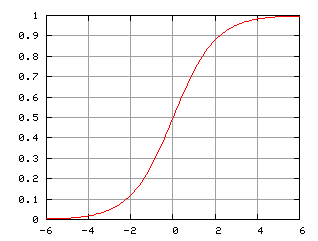
\includegraphics[width = 0.4\textwidth]{img/EcuacionLogistica.png}
\caption{Gráfica de $P(t) = \frac{1}{1+e^{-t}}$}
\label{fig:EcLogistica}
\end{figure}

\end{frame}

\subsection{Procesos de Verhulst.}

\begin{frame}
\framesubtitle{Modelo}
\begin{definition}[Proceso de Verhulst]
Modelo matemático que representa el desarrollo del número de individuos de una población a lo largo del tiempo.
\end{definition}

\uncover<2->{\textbf{Descripción del modelo}}
\begin{itemize}[<+(1)->]
\item Ratio de crecimiento
\[R=\frac{x_{n+1}-x_n}{x_n}\]

\item Si $R=r$ constante
\[x_{n+1} = f(x_n) = (1+r)x_n\]
lo que os lleva a
\[x_n = (1+r)^nx_0\]

\item Verhulst mejora el modelo con
\[R=r(1-x_n)\]
obteniendo
\begin{equation}\label{eq:Verhulst}
x_{n+1} = f(x_n) = (1+r)x_n - rx_n^2
\end{equation}
\end{itemize}
\end{frame}

\begin{frame}
\framesubtitle{Puntos fijos}

\begin{block}{Punto fijo}
Un punto fijo de una función $f$ es aquel tal que
\[x=f(x)\]
\end{block}

\begin{itemize}
\item El punto fijo $x_0=0$ es inestable.
\item El punto fijo $x_0=1$ requiere estudio
\begin{itemize}
\item Definimos el error
\[δ_n = x_n-1\]
\item Linealizando la ecuación \eqref{eq:Verhulst} tenemos
\[δ_{n+1} = (1-r)δ_n\]
\item Vemos que la estabilidad depende de $r$.
\end{itemize}
\end{itemize}
\end{frame}

\begin{frame}
\framesubtitle{Estabilidad según $r$}

\begin{minipage}{0.32\textwidth}
\begin{figure}[hbtp]
\centering
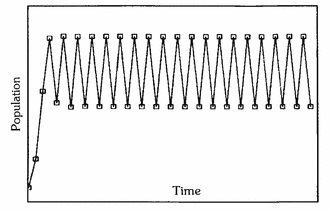
\includegraphics[width = \textwidth]{img/r2_3.png}
\caption{Evolución de la población con $r=2.3$}
\label{fig:r2_3}
\end{figure}
\end{minipage}
\begin{minipage}{0.32\textwidth}
\begin{figure}[hbtp]
\centering
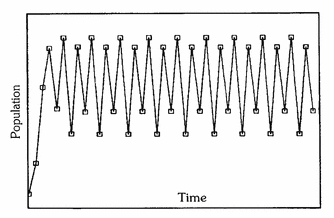
\includegraphics[width = \textwidth]{img/r2_5.png}
\caption{Evolución de la población con $r=2.5$}
\label{fig:r2_5}
\end{figure}
\end{minipage}
\begin{minipage}{0.32\textwidth}
\begin{figure}[hbtp]
\centering
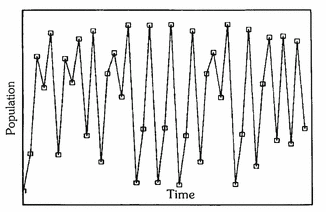
\includegraphics[width = \textwidth]{img/r3.png}
\caption{Evolución de la población con $r=3$}
\label{fig:r3}
\end{figure}
\end{minipage}
\end{frame}

\begin{frame}
\framesubtitle{Estabilidad}
\begin{figure}[hbtp]
\centering
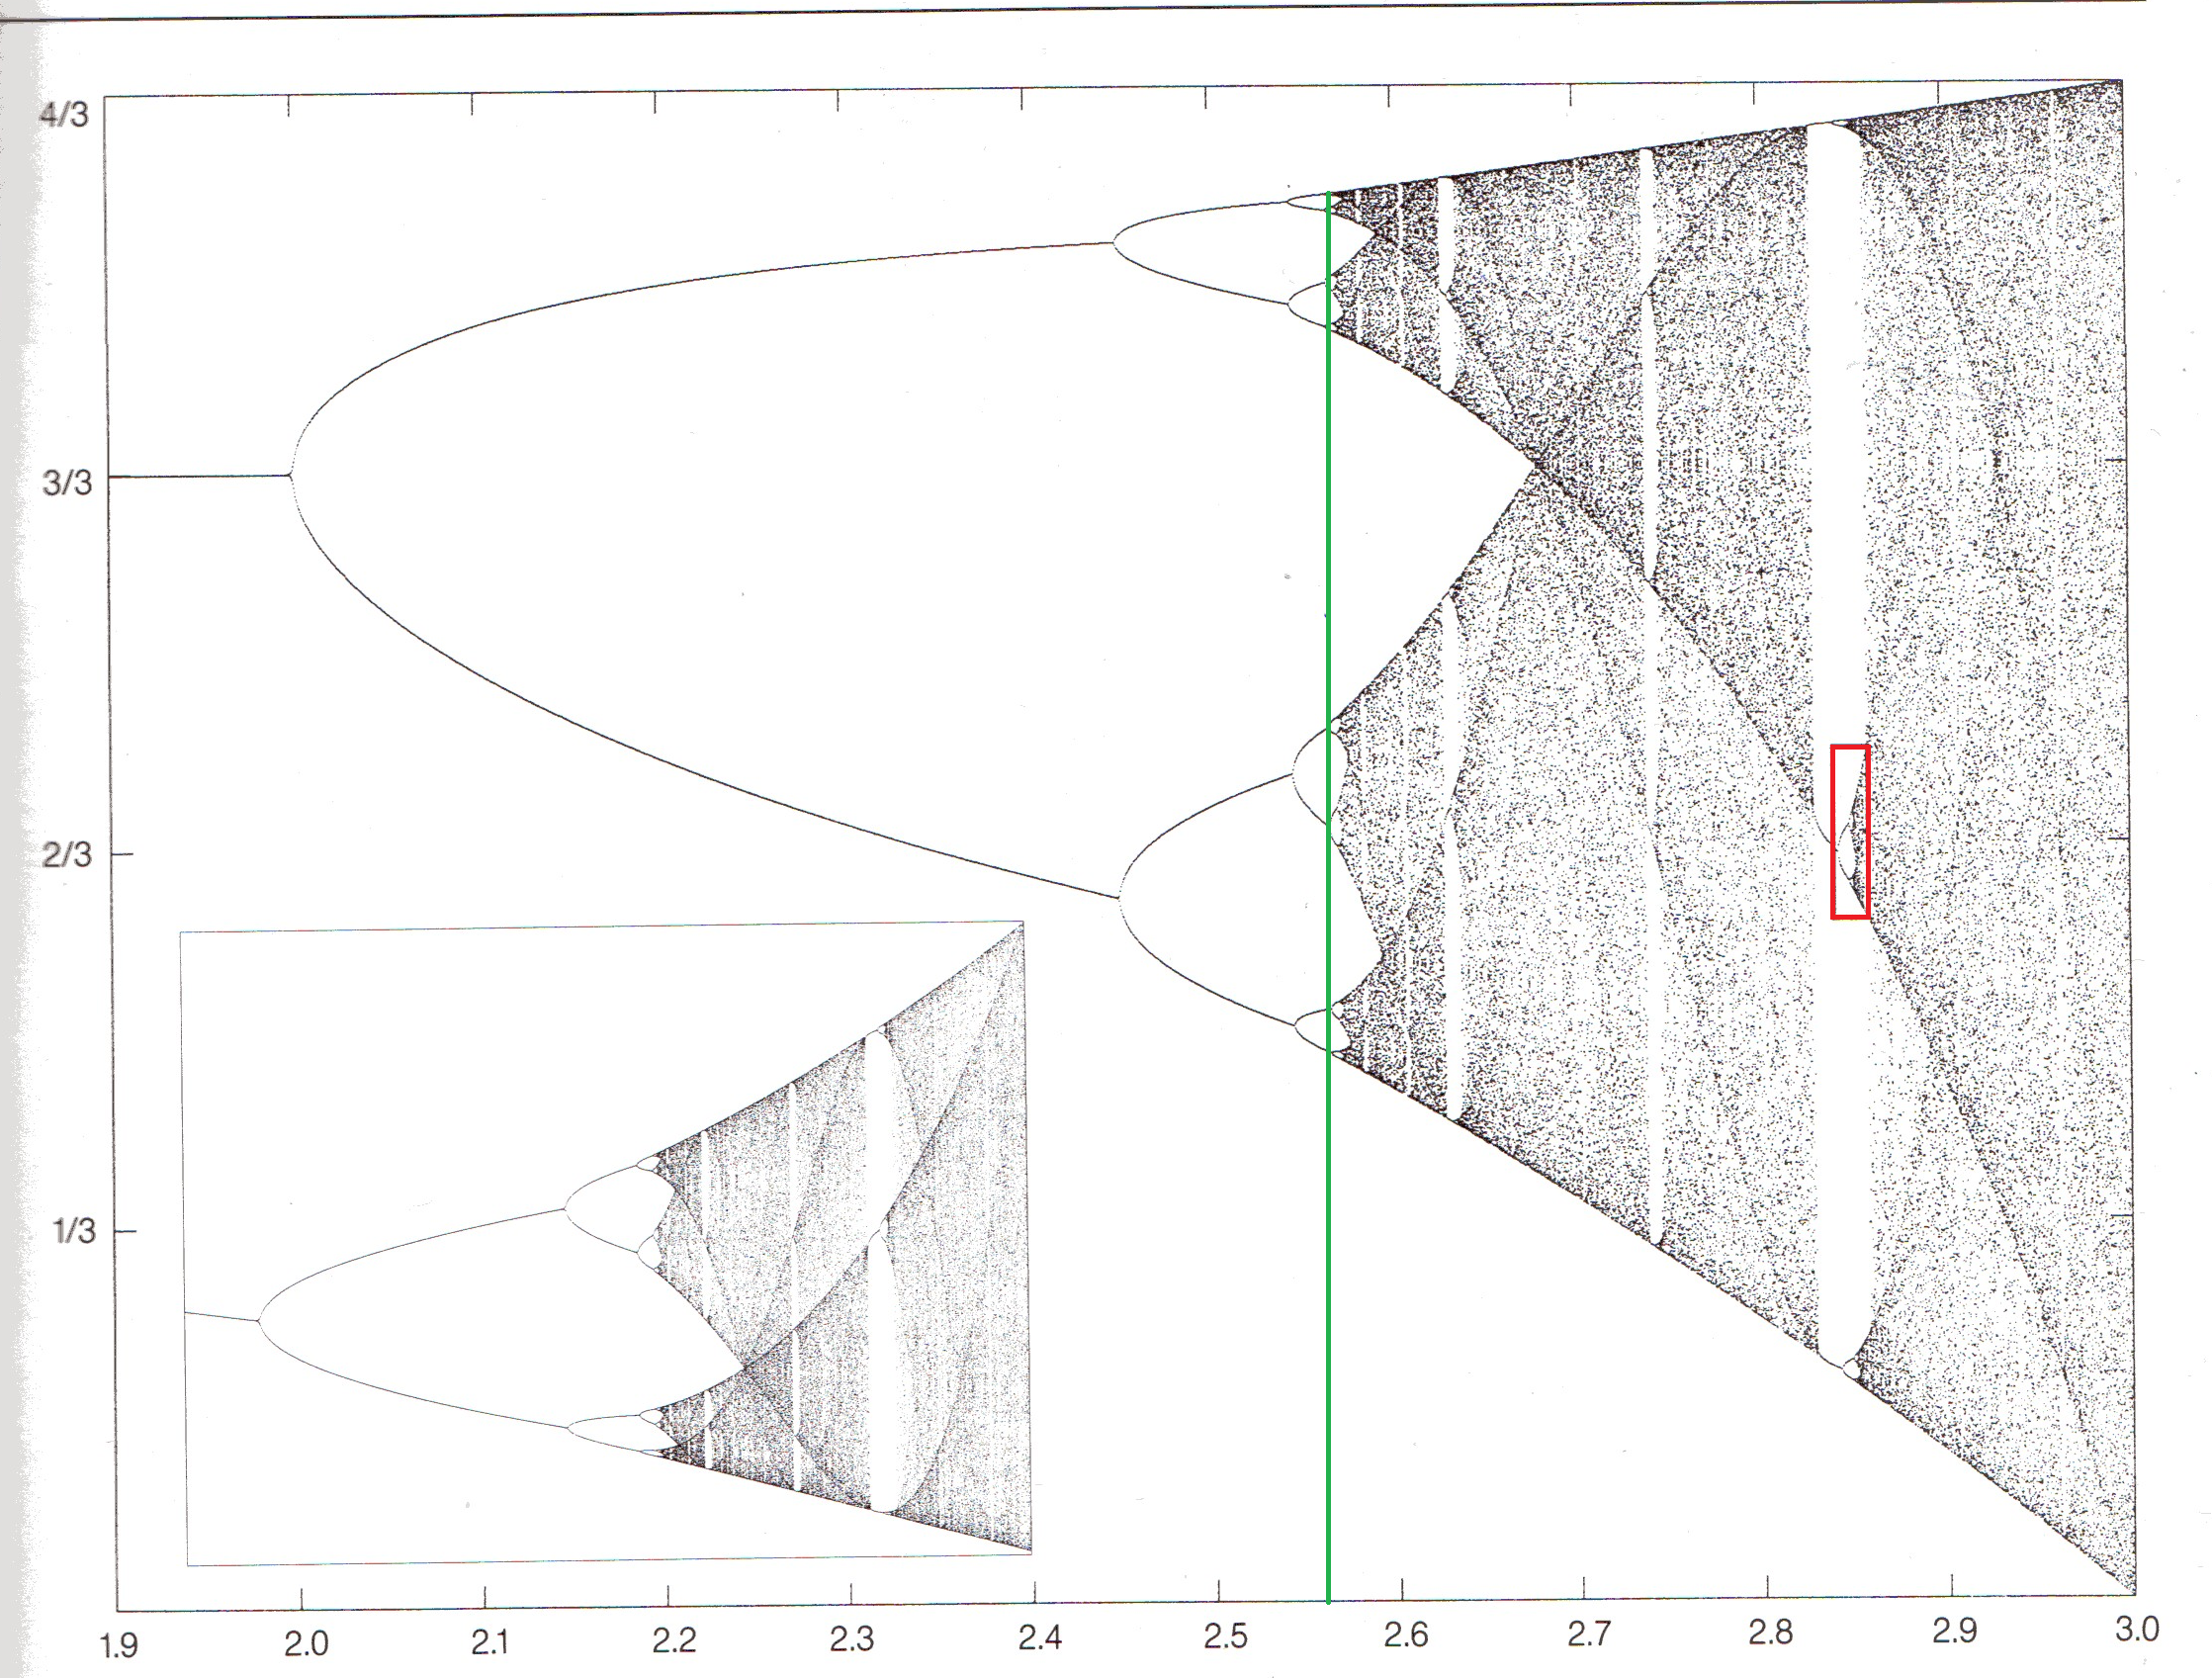
\includegraphics[width = 0.7 \textwidth]{img/verhulst6.png}
\caption{Visión global}
\label{fig:global}
\end{figure}
\end{frame}

\subsection{Conjuntos de Julia y Mandelbrot}

\begin{frame}
\framesubtitle{Repaso de números complejos}

Es necesario tener claras las ideas básicas de los números complejos para hablar de los conjuntos de Julia y Mandelbrot.

\begin{itemize}
\item Son números de la forma
\[z=a +bi\]
donde $a$ y $b$ son números reales e $i=\sqrt{-1}$
\item Se representan como puntos de un plano: \textbf{el plano complejo}

Cada número complejo tiene asociado un punto del plano y viceversa

\item Á menudo nos interesará considerar su módulo:
\[|z| = \sqrt{a^2+b^2}\]
\end{itemize}

\end{frame}

\subsubsection{Conjunto de Julia}

\begin{frame}
\begin{block}{Conjunto de Julia}
Familia de conjuntos fractales que se obtienen al estudiar el comportamiento de los números complejos al ser iterados por una función.

Iterando en la siguiente ecuación con $c$ constante obtenemos un ejemplo de conjunto de Julia

\begin{equation}
z_{n+1} = z_n^2+c \text{ siendo } c \text{ un número complejo}
\end{equation}\label{eq:Julia}
\end{block}

Para generarlo consideramos la iteración

\begin{minipage}{0.3\textwidth}
\[\begin{array}{l}
z_0=z_0\\
z_1=z_0^2+c \\
z_2 = z_1^2 + c \\
\vdots \\
z_{n+1} = z_n^2+c
\end{array}\]
\end{minipage}
\begin{minipage}{0.68\textwidth}
\begin{figure}[hbtp]
\centering
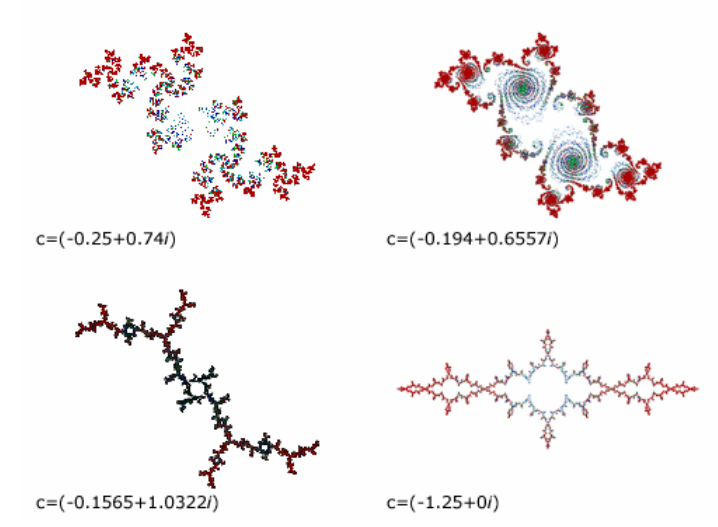
\includegraphics[width = 0.6\textwidth]{img/Julia_sets.png}
\caption{Ejemplos de conjuntos de Julia}
\label{fig:Julia}
\end{figure}
\end{minipage}
\end{frame}

\subsubsection{Conjunto de Mandelbrot}

\begin{frame}
\begin{block}{Conjunto de Mandelbrot}
Mandelbrot modifica el proceso iterativo de Julia haciendo variable el punto $c$ y fijando el punto $z_0=0$.
\end{block}

El conjunto de Mandelbrot es el conjunto de números complejos $c$ para los cuales la sucesión de puntos obtenida por el método iterativo:

\begin{minipage}{0.3\textwidth}
\[\begin{array}{l}
z_0=z_0\\
z_1=z_0^2+c \\
z_2 = z_1^2 + c \\
\vdots \\
z_{n+1} = z_n^2+c
\end{array}\]
no tiende a infinito, es decir, está acotada.
\end{minipage}
\begin{minipage}{0.68\textwidth}
\begin{figure}[hbtp]
\centering
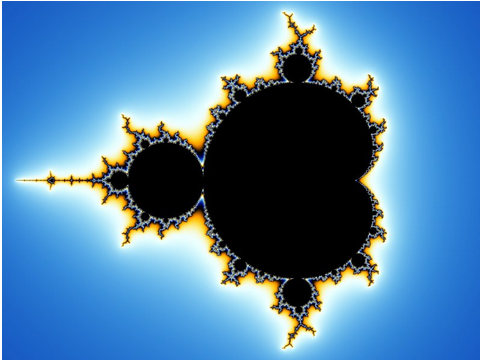
\includegraphics[width = 0.6\textwidth]{img/Mandelbrot_set.png}
\caption{Conjunto de Mandelbrot}
\label{fig:Mandelbrot}
\end{figure}
\end{minipage}
\end{frame}

\subsection{Fractales, dimensión de Hausdorlf y dimensión fractal}

\begin{frame}
\begin{itemize}
\item El término fractal fue propuesto por el matemático \textbf{Benoit Mandelbrot} en 1975, procedente del latin ``Fractus'' que significa ``fracturado''.
\item Recordemos que en la figura \ref{fig:Mandelbrot} la diferencia entre los distintos colores mostrados se debía a la convergencia o no de los diferentes puntos del plano al aplicarles la ecuación de Mandelbrot.
\item La relación entre el caos y los fractales se da en la frontera del dibujo.
\end{itemize}

\begin{minipage}{0.48\textwidth}
\begin{figure}[hbtp]
\centering
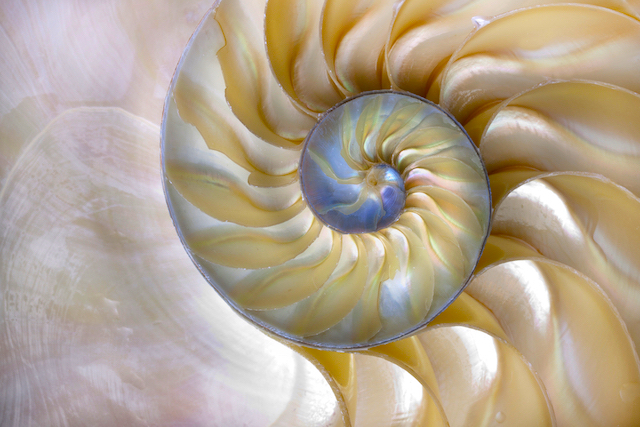
\includegraphics[width = 0.6\textwidth]{img/concha.jpg}
\caption{Concha de un molusco}
\label{fig:concha}
\end{figure}
\end{minipage}
\begin{minipage}{0.48\textwidth}
\begin{figure}[hbtp]
\centering
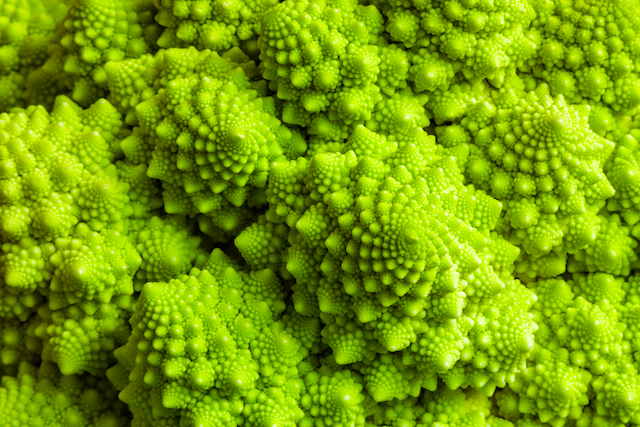
\includegraphics[width = 0.6\textwidth]{img/brocoli.jpg}
\caption{Trozo de brocoli al que se ha aplicado zoom}
\label{fig:brocoli}
\end{figure}
\end{minipage}

\begin{itemize}
\item La existencia de los fractales en la vida cotidiana se debe a la gran capacidad de comprimir información que tienen asociada.
\item Definición recursiva de árbol.
\end{itemize}

\end{frame}

\subsubsection{Dimensión de Hausdorff y dimensión fractal}

\begin{frame}
\begin{itemize}
\item La \textbf{dimensión topológica} de un cierto objeto en un espacio es $d$ si y sólo si cada punto del objeto se puede \emph{desconectar} (es decir, quitar uno o varios puntos dejando el objeto inconexo) del resto por un conjunto de dimension $d-1$.

\item Todas estas dimensiones son enteras

\item Los fractales tienen dimensión topológica entera pero se comportan como objetos de dimensión mayor.

\item Surge la dimensión de Hausdorff
\end{itemize}

\begin{block}{Dimensión de Hausdorff}
De nuevo, intuitivamente, la dimensión de Hausdorff nos dice cómo el objeto en cuestión llena el espacio en el que está inmerso. Para ellos recubriremos la figura con \emph{bolas} de radio $r$. La razón entre el número de bolas que necesitemos $N(r)$ y $ln(\frac{1}{r})$ es la dimensión fractal de nuestro objeto. Esto es,

\begin{equation}
D = \frac{N(r)}{ln(\frac{1}{r})}
\end{equation}

\end{block}
\end{frame}

\subsubsection{Ejemplos}
\begin{frame}
\begin{figure}[hbtp]
\centering
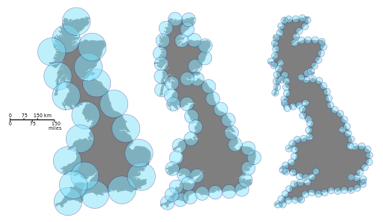
\includegraphics[width = 0.35\textwidth]{img/GB.png}
\caption{Medida fractal de la línea de costa de Gran Bretaña}
\label{fig:gb}
\end{figure}

\begin{figure}[hbtp]
\footnotesize
\begin{tabular}{|c|c|c|}
  \hline
  \textbf{Valor exacto} & \textbf{Valor aproximado} & \textbf{Nombre}   \\\hline
  $\frac{log(2)}{log(3)}$ & 0.6309 & Conjunto de Cantor \\
  Medida (recuento de cajas) & 1,2 & Conjunto de Julia \emph{Dendrita} \\
  $\log\left(\frac{1+\sqrt[3]{73-6\sqrt{87}}+\sqrt[3]{73+6\sqrt{87}}}{3}\right)\cdot \frac{1}{\log(2)}$ & 1,5236 & Frontera de la curva Dragón \\
  $3\frac{\log(\phi)}{\log(1+\sqrt{2})}$ & 1,6379 & Fractal de Fibonacci \\
  2 & 2 & Frontera del Conjunto de Mandelbrot \\
  Medido & 1,24 & Línea de costa de Gran Bretaña \\
  Medido & 1,52 & Línea de costa de Noruega \\
  \hline
\end{tabular}
\normalsize
\caption{Ejemplos de conjuntos con dimensión fractal}
\label{tab:ejemplos}
\end{figure}
\end{frame}

\subsection{Polvo de Cantor}

\begin{frame}
\begin{block}{Polvo de Cantor}
Se denomina Polvo de Cantor al fractal resultante de iterar sobre el conjunto de cantor en dos dimensiones.
\end{block}

\begin{block}{Conjunto de Cantor}
Conjunto construido mediante el siguiente proceso:

\begin{enumerate}
\item Tomamos el intervalo [0,1], lo dividimos en 3 intervalos iguales y eliminamos el intervalo central

\item Volvemos al paso 1 sobre cada uno de los dos conjuntos restantes.
\end{enumerate}

La imagen \ref{fig:conjuntoCantor} ilustra la construcción de este conjunto.
\end{block}

\begin{figure}[hbtp]
\centering
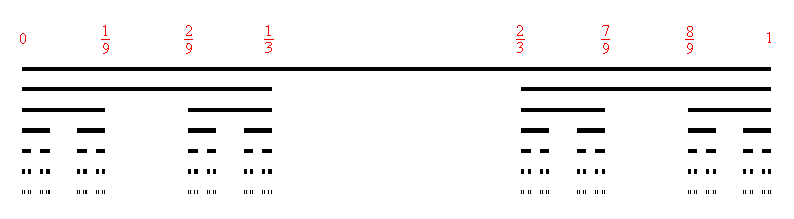
\includegraphics[width = 0.7\textwidth]{img/conjuntoCantor.png}
\caption{Primeras etapas del proceso de construcción del conjunto de Cantor}
\label{fig:conjuntoCantor}
\end{figure}

\end{frame}

\section{Sistemas continuos}
\subsection{Sistemas dinámicos deterministas, ecuaciones diferenciales}
\begin{frame}
\framesubtitle{Introducción}

\textbf{Comparación con ecuacines en diferencias:}
\begin{itemize}
\item La diferencia con los sistemas dinámicos en diferencias se debe a la continuidad de las variables
\item Expresamos los incrementos como derivadas
\item Obtenemos \textbf{ecuaciones diferenciales}
\end{itemize}

\begin{block}{Ecuación diferencial}
Una ecuación diferencial es una fórmula matemática que relaciona una función con sus derivadas.

Por ejemplo
\[y'(x) = y(x) \implies y(x) = e^{x+c}\]
\end{block}
\end{frame}

\begin{frame}
\framesubtitle{Ecuación del calor}

\begin{block}{Ecuación del calor}
La ecuación del calor es una importante ecuación diferencial en derivadas parciales del tipo parabólica que describe la distribución del calor (o variaciones de la temperatura) en una región a lo largo del transcurso del tiempo.
\end{block}

\textbf{Modelización del problema}
\begin{itemize}
\item La variable $t$ es el tiempo
\item Definimos $x(t)$ como la diferencia de temperatura en todo instante $t$
\item $x'(t)$ nos da la variación de temperatura en todo instante $t$
\item \textbf{Teoría:} La tasa de cambio de temperatura es inversamente proporcional a la diferencia de temperatura
\end{itemize}

La ecuación que modeliza este fenómeno es:
\begin{equation}
x'(t) = ax(t)~~~con~~ a<0
\end{equation}

Cuya solución viene dada por:
\begin{equation}
x(t) = c\cdot e^{at}
\end{equation}
\end{frame}

\begin{frame}
\framesubtitle{Péndulo}
\begin{block}{Movimiento del péndulo}
Queremos estudiar el movimiento de un péndulo que tiene en su extremo un peso y que cuelga de un soporte que limita su movimiento a lo largo de un círculo.
\end{block}

\textbf{Modelización del sistema}
\begin{itemize}
\item La variable $t$ es el tiempo.
\item Definimos $x(t)$ como la posición angular del péndulo en todo instante $t$.
\item La función $x'(t)$ mide la velocidad angular del péndulo.
\item La función $x''(t)$ mide la aceleración angular del péndulo en todo instante $t$
\end{itemize}

La ecuación que modeliza este fenómeno es:
\begin{equation}
x''(t) = -\sin x(t)
\end{equation}

Se trata de una ecuación de \emph{segundo orden} y es una de las más importantes en ciencia.
\end{frame}

\begin{frame}
\framesubtitle{Clasificación de Ecuaciones Diferenciales Ordinarias}
\begin{itemize}
\item Según el orden de las derivadas que aparezcan en la expresión:
  \begin{itemize}
  \item Primer orden
  \item Segundo orden
  \item ...
  \end{itemize}
\item Según la relación entre la función $x$ y sus derivadas
  \begin{itemize}
  \item Lineales
  \item No lineales
  \end{itemize}
\item Según si aparece explicítamente la variable $t$ en la ecuación
  \begin{itemize}
  \item Autónomas
  \item No autónomas
  \end{itemize}
\end{itemize}
\end{frame}

\begin{frame}
\framesubtitle{Dependencia del dato inicial: Caos}

\begin{block}{Dependencia del dato inicial}
Siempre es necesario conocer un dato inicial a fin de determinar con exactitud la solución de la ecuación. Sin embargo, en ocasiones, pequeños errores al medir este dato inicial pueden dar lugar a grandes cambios en el sistema.
\end{block}

\begin{minipage}{0.48\textwidth}
\begin{center}
\begin{tikzpicture}
\begin{axis}[xmin=-1, xmax=1, samples=50, width=6cm, height=6cm, cycle list name=color list]
  \addplot (x,-7*e^x);
  \addplot (x,-6*e^x);
  \addplot (x,-5*e^x);
  \addplot (x,-3*e^x);
  \addplot (x,4*e^x);
  \addplot (x,-3*e^x);
  \addplot (x,-2*e^x);
  \addplot (x,-1*e^x);
  \addplot (x,e^x);
  \addplot (x,2*e^x);
  \addplot (x,3*e^x);
  \addplot (x,4*e^x);
  \addplot (x,5*e^x);
  \addplot (x,6*e^x);
  \addplot (x,7*e^x);
\end{axis}
\end{tikzpicture}
\captionof{figure}{Familia de funciones de la forma $x(t)=x(0)e^t$}
\end{center}
\end{minipage}
\begin{minipage}{0.48\textwidth}
\begin{center}
\begin{tikzpicture}
\begin{axis}[xmin=-1, xmax=1, samples=50, width=6cm, height=6cm, cycle list name=color list]
  \addplot (x,-7*e^-x);
  \addplot (x,-6*e^-x);
  \addplot (x,-5*e^-x);
  \addplot (x,-3*e^-x);
  \addplot (x,4*e^-x);
  \addplot (x,-3*e^-x);
  \addplot (x,-2*e^-x);
  \addplot (x,-1*e^-x);
  \addplot (x,e^-x);
  \addplot (x,2*e^-x);
  \addplot (x,3*e^-x);
  \addplot (x,4*e^-x);
  \addplot (x,5*e^-x);
  \addplot (x,6*e^-x);
  \addplot (x,7*e^-x);
\end{axis}
\end{tikzpicture}
\captionof{figure}{Familia de funciones de la forma $x(t)=x(0)e^{-t}$}
\end{center}
\end{minipage}
\end{frame}

\subsection{Espacio de estados/fases}

\begin{frame}
\begin{itemize}
\item A menudo no es nada sencillo obtener la solución de una ecuación diferencial.
\item En matemáticas hay una asignatura completa dedicada a la comprensión de estas ecuaciones.
\item Sin embargo puede estudiarse la tendencia general de la solución.
\item Para ello empleamos los \textbf{diagrama de fases}
\end{itemize}

\textbf{Consideramos un problema general $y'(t)=f(y(t))$}
\begin{figure}[hbtp]
\centering
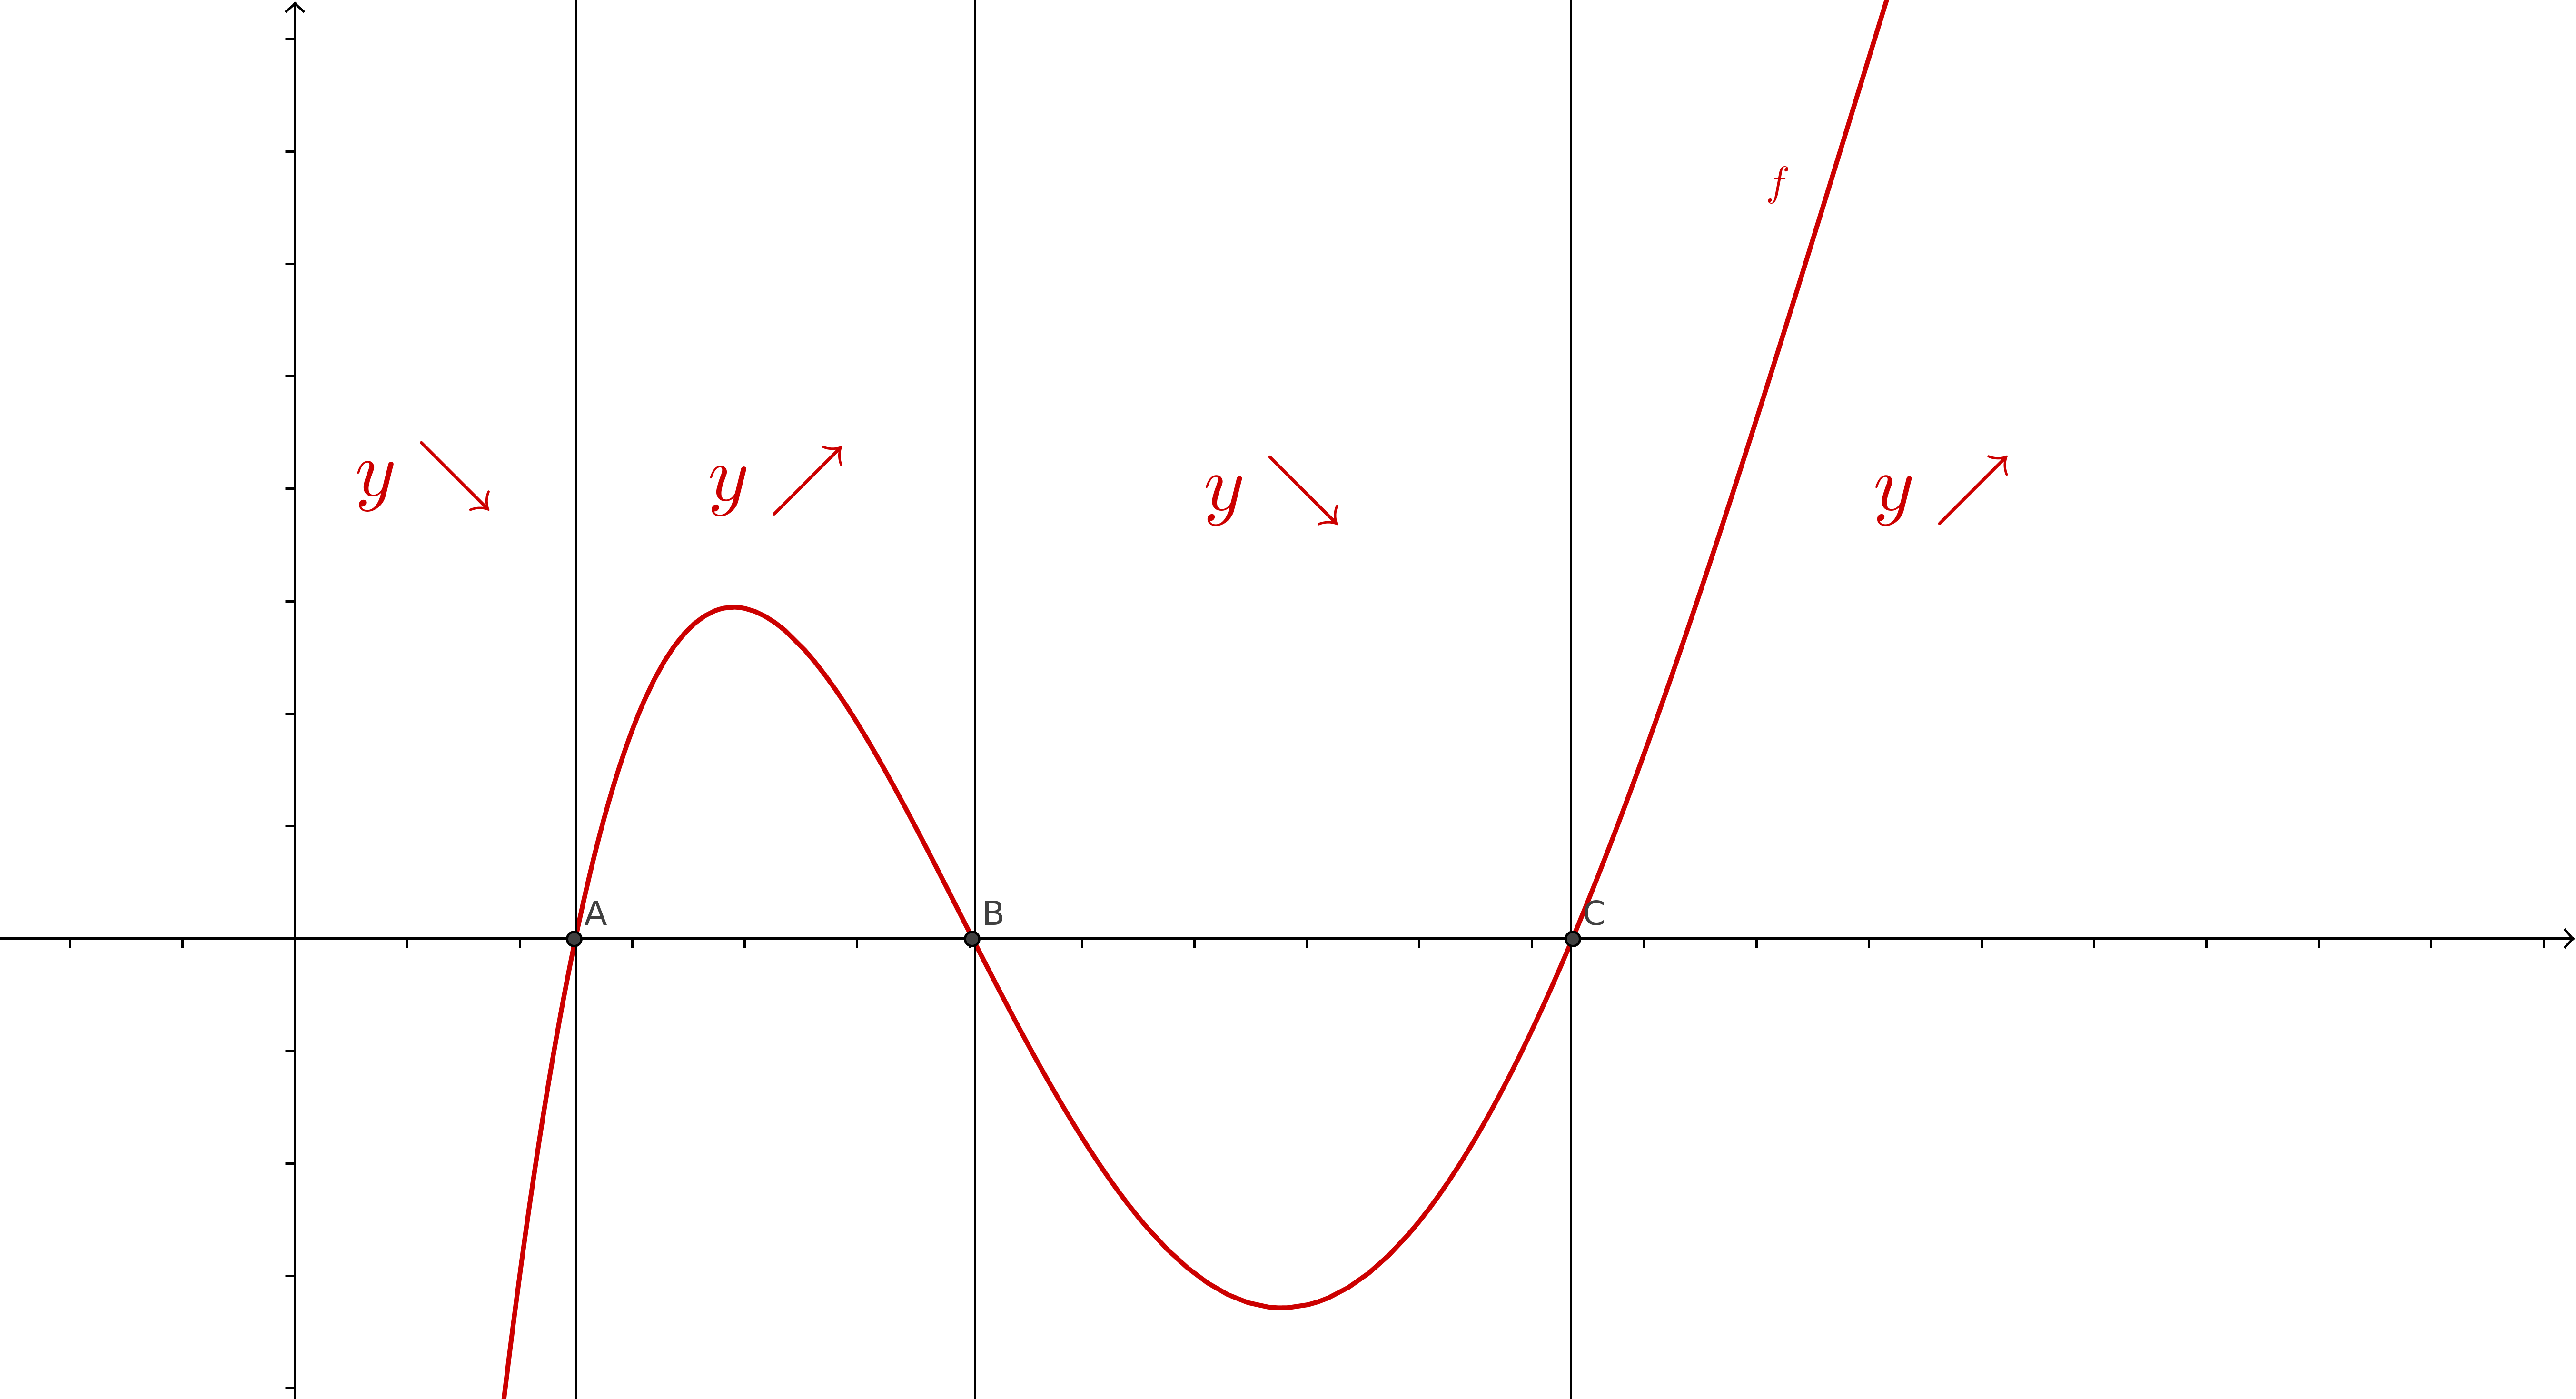
\includegraphics[width = 0.6\textwidth]{img/propiedades-autonomas.png}
\end{figure}

\begin{figure}[hbtp]
\centering
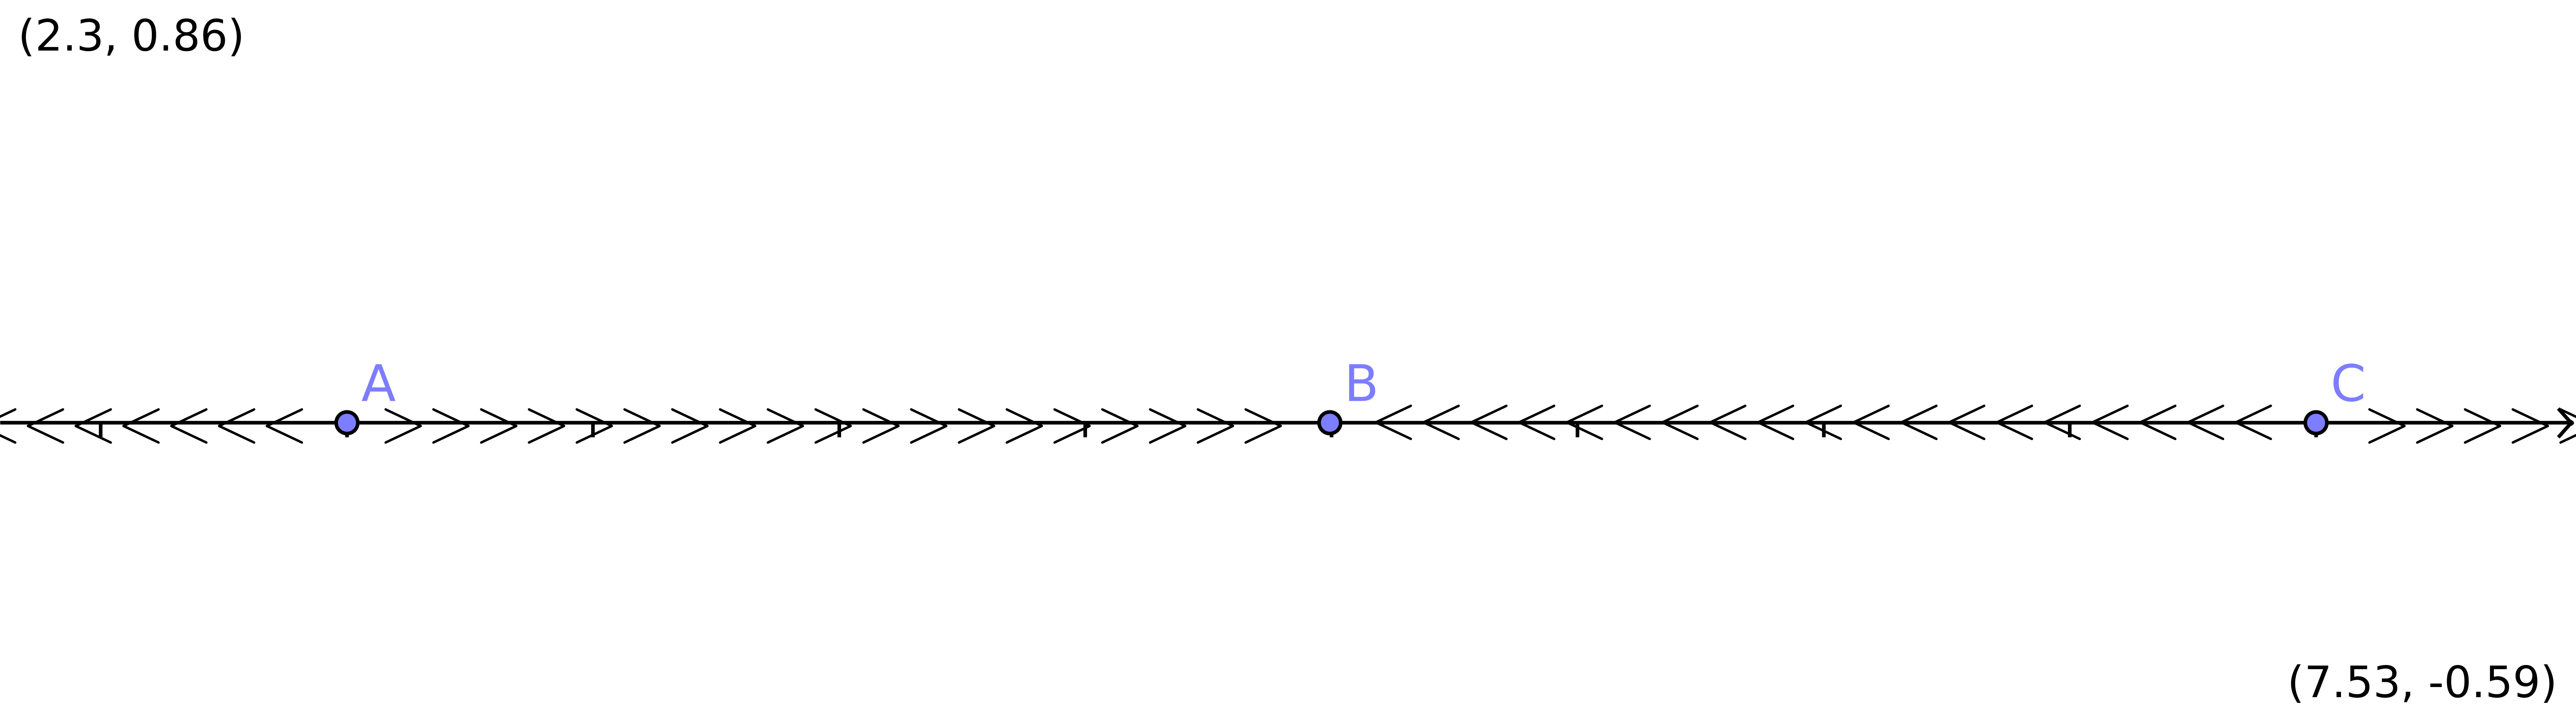
\includegraphics[width = 0.6\textwidth]{img/diagrama-fases.png}
\end{figure}

\end{frame}
\subsection{Algunos ejemplos}

\begin{frame}
\begin{example}
Consideremos de nuevo la E.D.O. (ecuación diferencial ordinaria):
\begin{equation}
x'(t) =ax(t)
\end{equation}
Cuya solución era:
\begin{equation}
x(t) =ce^{at}
\end{equation}
\begin{minipage}{0.48\textwidth}
\begin{center}
\begin{figure}[hbtp]
\centering
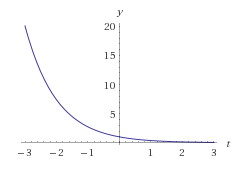
\includegraphics[width = 0.6\textwidth]{img/exp.png}
\caption{Caso $a=-1$: $x(t)=ce^{-t}$}
Error despreciable
\end{figure}
\end{center}
\end{minipage}
\begin{minipage}{0.48\textwidth}
\begin{center}
\begin{figure}[hbtp]
\centering
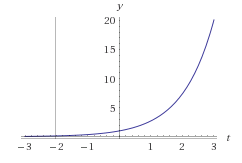
\includegraphics[width = 0.6\textwidth]{img/exp2.png}
\caption{Caso $a=1$: $x(t)=ce^{t}$}
Error NO despreciable
\end{figure}
\end{center}
\end{minipage}
\end{example}
\end{frame}

\subsection{Ecuaciones diferenciales no lineales}
\begin{frame}
\textbf{Problema:} La mayoría no pueden ser resueltos de manera explícita. Usaremos propiedades \textbf{cualitativas} de las soluciones.

\begin{example}
\textbf{Función logística de la población}
\begin{equation}
x'(t) = a\cdot x(t)\left(1-\frac{x(t)}{K}\right)~~~~con~~a>0~~y~~K>0
\end{equation}
\end{example}
\end{frame}

\begin{frame}
%Grafica que deberia aparecer tambien en el pdf
\begin{figure}[hbtp]
\centering
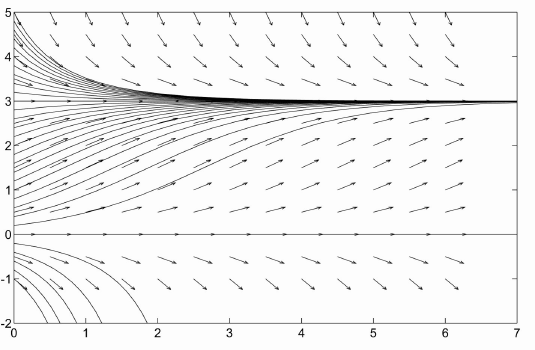
\includegraphics[width = 0.4\textwidth]{img/poblacion.png}
\caption{Soluciones de la ecuación logística diferencial}
\end{figure}\label{fig:poblacion}

\begin{itemize}
\item \textbf{Soluciones de equilibrio:} $x(t) = 0$ y $x(t)=1$
\item $x(t) = 0$ es un \textbf{sumidero} mientras que $x(t)=1$ es una \textbf{fuente}.
\item La población crecerá siempre que la problación inicial sea positiva y estrictamente menor que K.
\item Las soluciones que corresponden a valores negativos de la población \emph{explotan}. Afortunadamente, no tienen sentido físico.
\end{itemize}
\end{frame}

\begin{frame}
\begin{block}{Tres conceptos importantes}
\begin{itemize}
\item Existencia de solución
\item Unicidad de la solución
\item Dependencia continua $\neq$ Dependencia \emph{sensible}
\end{itemize}
\end{block}
\textbf{Observación}: La \emph{dependencia sensible} o \textbf{efecto mariposa} es la característica más importante de los \textbf{sistemas caóticos}.
\end{frame}

\subsection{Sistemas disipativos: atractores}
\begin{frame}
\begin{figure}[hbtp]
\centering
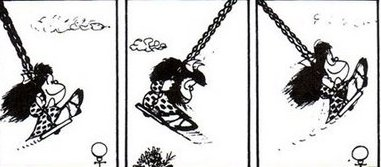
\includegraphics[width = 0.6\textwidth]{img/columpio.jpg}
\caption{Un columpio es un sistema disipativo}
\end{figure}
\begin{definition}[Atractor]
Conjunto hacia el que todas las trayectorias cercanas convergen.
\begin{itemize}
\item Es invariante, toda trayectoria que empiece en el conjunto nunca sale de él.
\item Existe un conjunto abierto $U$ que contiene al atractor de modo que toda trayectoria que comience en $U$ acaba en el atractor.
\item Un atractor es el conjunto más pequeño que cumple estas propiedades.
\end{itemize}
\end{definition}
\end{frame}

\begin{frame}
\begin{example}
Si consideramos el sistema bidimensional
\[\begin{array}{l}
x'(t) = x(t)-x^3(t) \\
y'(t) = -y(t)
\end{array}\]
podemos ver fácilmente que su plano de fases será el mostrado en la figura \ref{fig:planoFasesAtractorEjemplo}.
\begin{figure}[H]
\centering
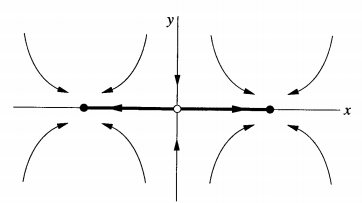
\includegraphics[width = 0.4\textwidth]{img/atractorExample.png}
\caption{Plano de fases asociado al sistema descrito en el ejemplo}
\label{fig:planoFasesAtractorEjemplo}
\end{figure}
El \textbf{atractor} sería el conjunto \[A=\{(\pm 1, 0)\}\]
\end{example}
\end{frame}
\begin{frame}
\begin{example}[El péndulo]
\begin{minipage}{0.48\textwidth}
\begin{center}
\begin{figure}[hbtp]
\centering
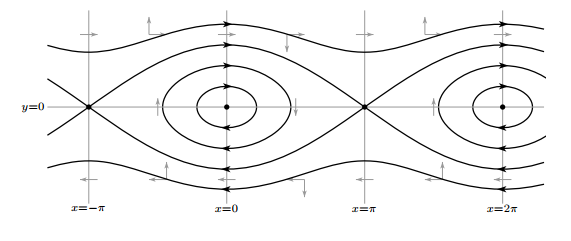
\includegraphics[width = 0.8\textwidth]{img/pend_simple.jpg}
\caption{Plano de fases del péndulo simple}
\end{figure}
\end{center}
\end{minipage}
\begin{minipage}{0.48\textwidth}
\begin{center}
\begin{figure}[hbtp]
\centering
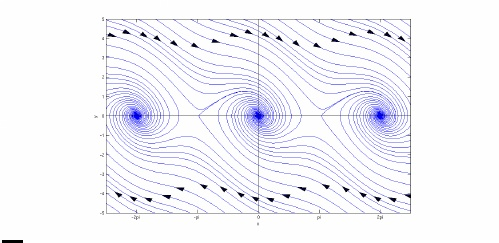
\includegraphics[width = 0.8\textwidth]{img/pend_amort.jpg}
\caption{Plano de fases del péndulo amortigüado}
\end{figure}
\end{center}
\end{minipage}
\end{example}
\end{frame}
\subsection{Flujos, compresibles o no}
\begin{frame}
\begin{definition}[Compresibilidad de un fluido]
Propiedad para disminuir su volumen al aplicar presión o compresión. Los gases son altamente \emph{compresibles} mientras que los líquidos son altamente \emph{incompresibles}.
\end{definition}
\begin{block}{}
Movimiento \textbf{estacionario}: Las condiciones de velocidad en un punto no cambian con el tiempo.
\begin{itemize}
\item Fluido viscoso
\item Baja velocidad de movimiento
\end{itemize}
Flujo \textbf{turbulento} o \textbf{caótico}: El movimiento se vuelve irregular y desordenado.
\begin{itemize}
\item Alta velocidad del flujo
\end{itemize}
\end{block}
\begin{figure}[hbtp]
\centering
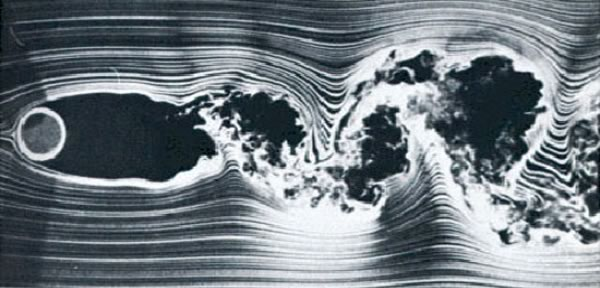
\includegraphics[width = 0.4\textwidth]{img/flujo_turb.jpg}
\caption{Flujo de un fluido}
\end{figure}
\end{frame}
\begin{frame}
\begin{block}{Enfoque Optimista}
El flujo turbulento es resultado de la ampliación de un movimiento que incluye tantas componentes de frecuencia que parece volverse desordenado y confuso. Existe una \textbf{estructura periódica} subyacente pero es demasiado compleja para seguirla.
\end{block}
\begin{block}{Teoría del Caos}
El movimiento turbulento tiene un \textbf{comportamiento completamente aperiódico}. Deja de ser susceptible de cualquier predicción. En general, 2 partículas que se muevan de forma parecida en el flujo en un tiempo dado pueden hallarse en estados de movimiento totalmente diferentes tras un lapso suficiente de tiempo.
\end{block}
\end{frame}
\subsection{Atractores extraños: caos}
\begin{frame}
\begin{definition}[Atractores extraños]
Llamamos \textbf{atractor extraño} a aquellos con \textbf{dimensión de Hausorff no entera} o fractal. También decimos que un atractor es extraño cuando su dinámica es \textbf{caótica}.
\end{definition}
\begin{block}{Propiedades}
\begin{itemize}
\item Órbitas irregulares
\item Las trayectorias divergen exponencialmente
\item EL espacio de fases es \emph{acotado}.
\end{itemize}
\end{block}
\end{frame}
\subsubsection{Ejemplos de atractores extraños: Mapa de Henón}
\begin{frame}
\begin{definition}[Mapa de Henón]
Es un sistema dinámico discreto en el tiempo y uno de los más estudiados cuando analizamos comportamientos caóticos.\newline
$\left.
\begin{array}{rcl}
x_{n+1} & = & 1-ax^2_n+y_n\\
y_{n+1}& =& bx_n
\end{array}\right\}$\newline
\end{definition}
\begin{figure}[hbtp]
\centering
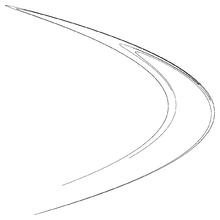
\includegraphics[width = 0.3\textwidth]{img/henon_clas.png}
\caption{Atractor de Henón para a=1.4 y b=0.3}
\label{fig:henon_clas}
\end{figure}
\end{frame}

\begin{frame}
\begin{block}{Mapa de Henón}
Supongamos $b=0.3$:
\begin{figure}[hbtp]
\centering
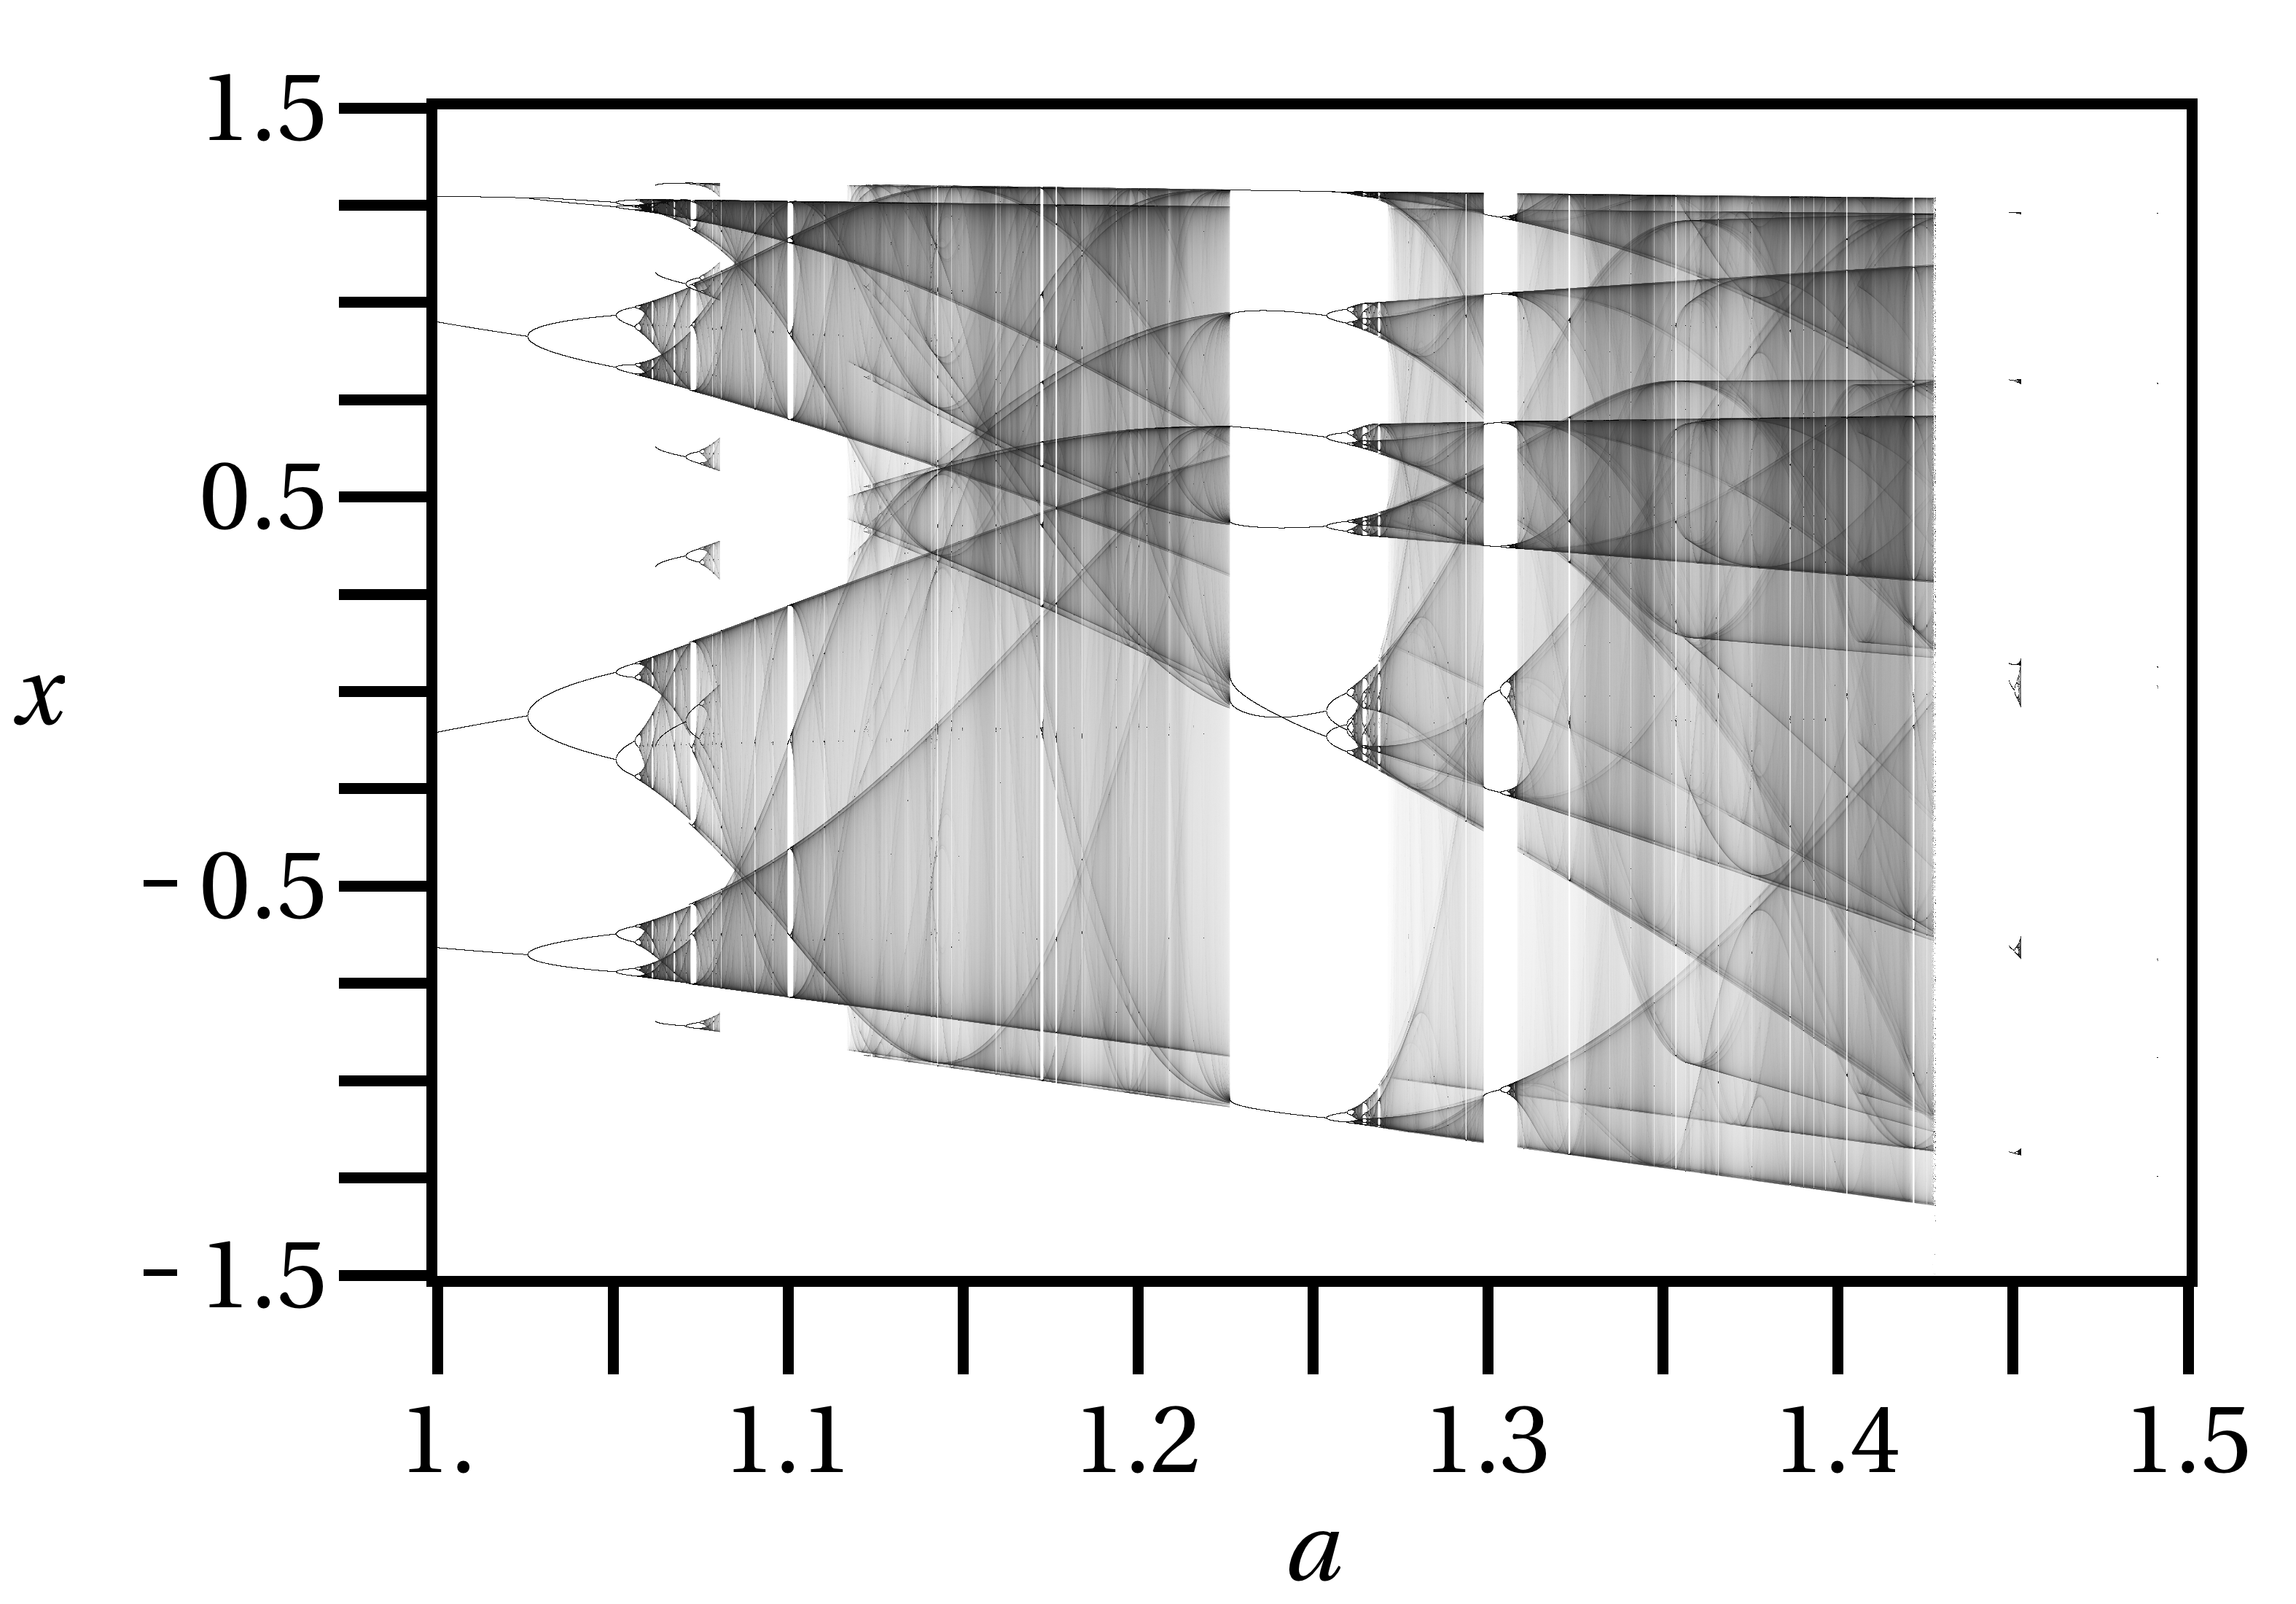
\includegraphics[width = 0.6\textwidth]{img/henon_orb.png}
\caption{Esquema de órbita para el mapa de Henón con b=0.3}
\label{fig:henon_orb}
\end{figure}
\end{block}
\end{frame}

\subsection{Ecuaciones de Lorenz}

\subsubsection{Introducción}
\begin{frame}
\begin{block}{Ecuaciones de Lorenz}
En 1963 Lorenz trató de desarrollar un modelo que permitiera predecir el clima.

El sistema descrito por Lorenz fue:
\[\begin{array}{l}
x'(t) = σ(y(t)-x(t)) \\
y'(t) = rx(t)-y(t)-x(t)y(t)\\
z'(t) = x(t)y(t)-bz(t)
\end{array}\]
donde σ es el \textbf{número de Prandtl}, que representa la viscosidad/conductividad térmica, $r$ es el \textbf{número de Rayleigh}, que representa la diferencia de temperatura entre base y tope y $b$ es la razón entre la longitud y altura del sistema.
\end{block}

\begin{itemize}
\item El sistema parecía ser muy simple (y por tanto útil)
\item Pero escondía un comporamiento realmente caótico.
\item Las soluciones daban lugar a una figura con ``forma de mariposa'' conocida hoy en día como \textbf{atractor extraño}.
\item Este atractor es un fractal con dimensión entre 2 y 3.
\end{itemize}
\end{frame}

\begin{frame}
\begin{figure}[hbtp]
\centering
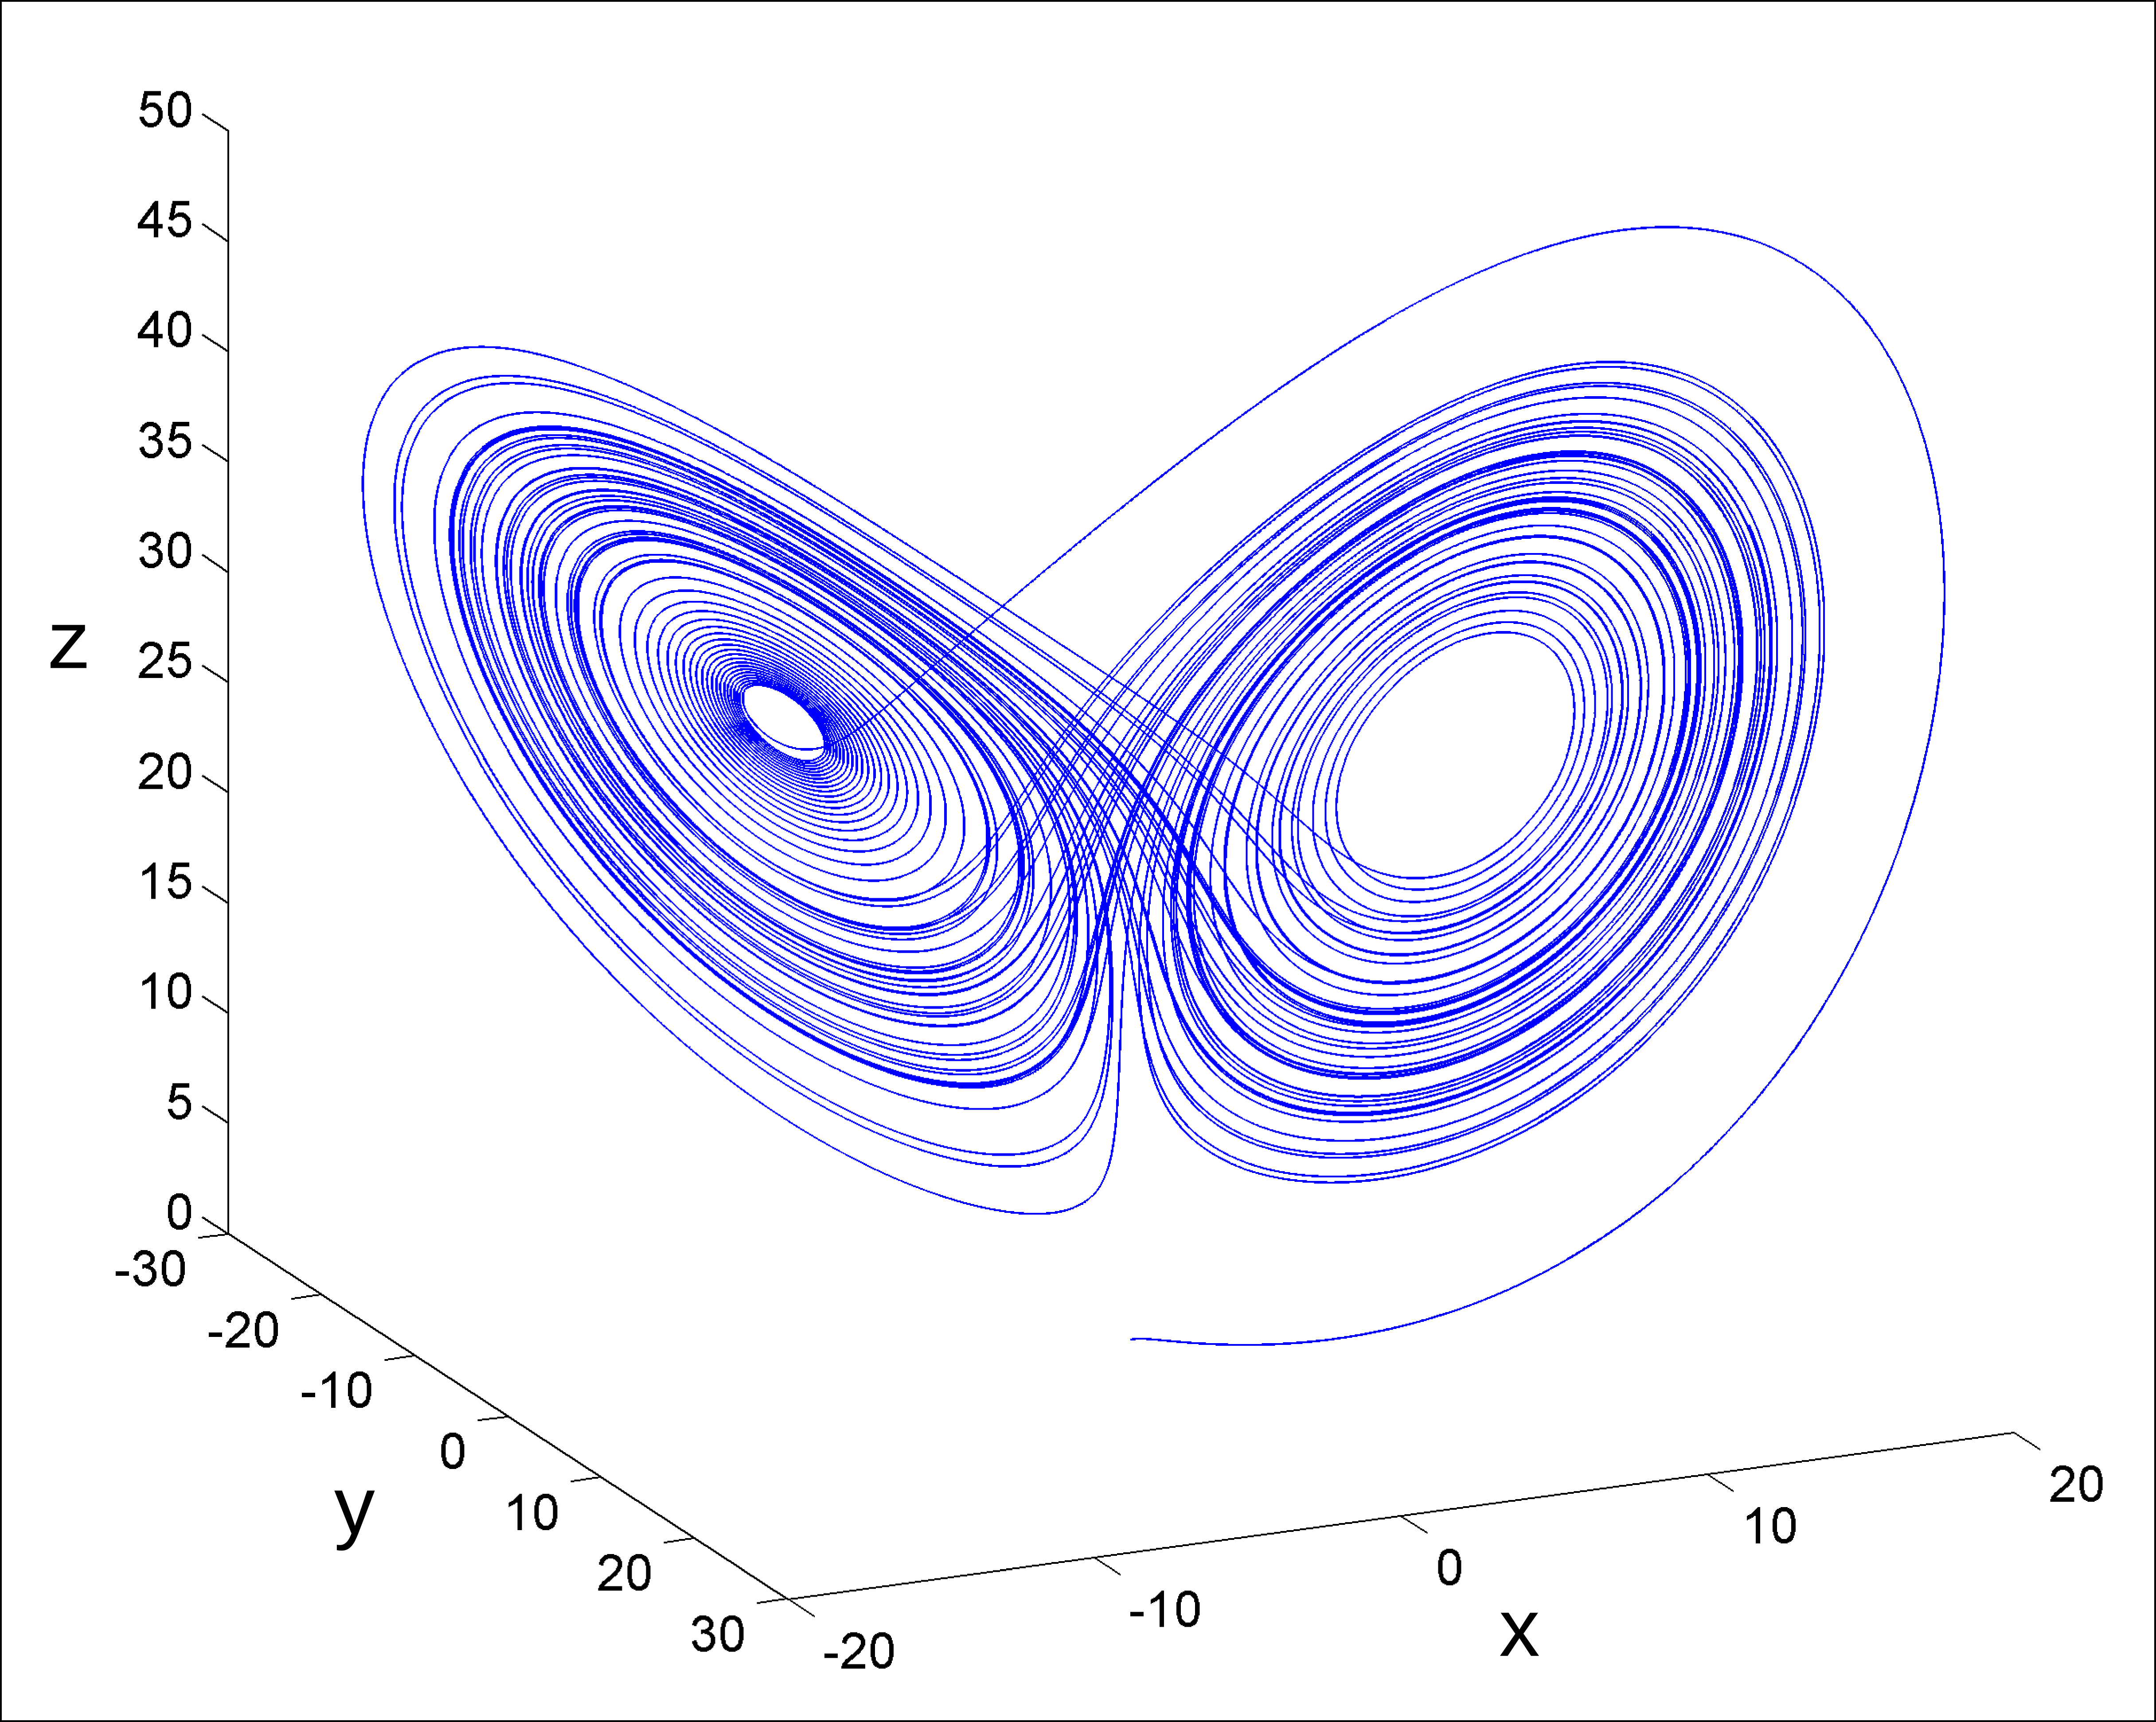
\includegraphics[width = 0.6\textwidth]{img/Lorenz.png}
\caption{Representación tridimensional de la solución de las ecuaciones de Lorenz}
\label{fig:Lorenz}
\end{figure}
\end{frame}

\subsubsection{Propiedades}
\begin{frame}
\begin{block}{Aparente paradoja}
Lorenz demostró que las soluciones no salían de una cierta región \emph{delimitada} y que, llegado a cierto punto, se veían atraídas hacia un conjunto de volumen cero.
\end{block}

\begin{itemize}
\item \textbf{No linearidad}
\item \textbf{Simetría}
Es decir, si $(x(t),y(t),z(t))$ es una solución también lo será $(-x(t),-y(t),z(t))$.
\[\begin{array}{l}
-x'(t) = -σ(y(t)-x(t)) \\
-y'(t) = -rx(t)+y(t)-x(t)y(t)\\
z'(t) = x(t)y(t)-bz(t)
\end{array}\]
\item \textbf{Puntos fijos}
\begin{itemize}
\item El $(0,0,0)$ siempre es punto fijo.
\item Según los parámetros tenemos el otro punto fijo:
\[\left(\pm \sqrt{b(r-1)},\pm \sqrt{b(r-1)},r-1\right) \text{ para } r>1\]
\item Definimos $C^+$ y $C^-$
\end{itemize}
\end{itemize}
\end{frame}

\begin{frame}
\begin{itemize}
\item \textbf{Contracción de volumen}

El sistema de Lorenz es \emph{disipativo}: el volumen en el plano de fases se contrae.

\begin{block}{Demostración}
Para cualquier sistema n-dimensional consideramos una superficie cerrada con un cierto volumen en el plano de fases.

\begin{figure}[hbtp]
\centering
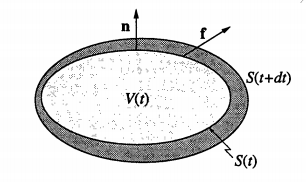
\includegraphics[width = 0.35\textwidth]{img/volumen2D.png}
\caption{Evolución con el tiempo de la superficie y del volumen contenido en su interior, siendo \textbf{n} el vector normal a la superfice $S(t)$}
\label{fig:volumen2D}
\end{figure}

El volumen varía según la ecuación:
\[V(t+dt)=V(t) + \int_S (f\cdot \text{\textbf{n}}\ dt)\ dA\]
\end{block}
\end{itemize}
\end{frame}

\begin{frame}
\begin{block}{Continuación}
Puesto que
\[V'(t)=\frac{V(t+dt)-V(t)}{dt} = \int_S f\cdot \text{\textbf{n}}\ dA\]

Aplicando el teorema de divergencia podemos reescribir la integral como:
\[V'(t) = \int_V \nabla \cdot f \ dV \]
siendo, para el sistema de Lorenz
\[\nabla \cdot f = \frac{\partial}{\partial x}[σ(x-y)] + \frac{\partial}{\partial y}[rx-y-xy] + \frac{\partial}{\partial z}[xy-bz] = -σ-1-b < 0\]

Puesto que la divergencia es constante, la ecuación de la derivada del volumen queda
\[V'(t) = -(σ+1+b)V(t) \implies V(t) = V(0)e^{-(σ+1+b)t}\]
con lo que queda claro que el volumen de crece de manera exponencial.
\end{block}
\end{frame}

\begin{frame}
\textbf{Respecto a la estabilidad en el origen:}

\begin{itemize}[<+(1)->]
\item \textbf{Estabilidad lineal del origen}

\begin{itemize}[<+(1)->]
\item Sistema linealizado
\[\begin{array}{l}
x'(t) = σ(y(t)-x(t)) \\
y'(t) = rx(t)-y(t)\\
z'(t) = -bz(t)
\end{array}\]
\item Ecuación matricial
\[\left(\begin{array}{l}
x'(t) \\ y'(t)
\end{array} \right) = \left(\begin{array}{cc}
-σ & σ \\ r & -1
\end{array} \right)\left(\begin{array}{l}
x(t) \\ y(t)
\end{array} \right)\]
\item La traza de la matriz es $τ=-σ-1<0$ y el determinante $Δ = σ(1-r)$.
\item Si $r>1$ el origen es un \emph{punto de silla} pueso que $Δ<0$
\item Si $r<1$ entonces nos encontramos ante un sumidero
\end{itemize}
\item \textbf{Estabilidad global del origen}

El origen es \textbf{globalmente estable} pues toda trayectoria con $r<1$ tiende al origen cuando $t$ lo hace a $\infty$
\end{itemize}
\end{frame}


\subsection{Órbitas caóticas y exponentes de Lyapunov}

\begin{frame}
\framesubtitle{Definición}
\textbf{El concepto de equilibrio inestable es muy común en física}

\begin{example}
Aunque en teoría podemos colocar una pelota en el pico de una montaña sin que se mueva, en la práctica esto es imposible.

El estado de equilibrio estático es \textbf{inestable}
\end{example}

Un comportamiento muy común en algunos sistemas dinámicos es pasar de un estado de equilibrio inestable a otro estable.

\begin{block}{Órbitas caóticas}
Las órbitas caóticas son aquellas que permanecen siempre en un estado inestable, sin llegar a converger o ser atraídas hacia níngun estado estático o periódico estable.

Esta irregularidad es cuantificada mediante los \textbf{números de Lyapunov} y los \textbf{exponentes de Lyapunov}.
\end{block}

\begin{block}{Número de Lyapunov}
Informalmente, diremos que el \textbf{número de Lyapunov} es la tasa o razón media a la que los puntos divergen a lo largo de la órbita. Diremos que el \textbf{exponente de Lyapunov} es el logaritmo natural del número de Lyapunov.
\end{block}

\end{frame}

\begin{frame}
\framesubtitle{Ejemplo numérico}

\begin{itemize}
\item Encontramos \emph{caos} cuando los coeficientes de Lyapunov de nuestro sistema dinámico son mayores que 1.
\end{itemize}

\begin{block}{Exponente de Lyapunov (definición formal)}
Dado un dato inicial $x_0$ consideramos un dato cercano $x_0+ε_0$, como ya hicimos en el ejemplo \ref{example:Julia} siendo la separación $ε_0$ extremadamente pequeña.

Sea $ε_n$ la separación tras $n$ iteraciones, si se da la relación $|ε_n|\approx e^{n\cdot λ}|ε_0|$, decimos que λ es el \textbf{exponente de Lyapunov}.
\end{block}

\begin{example}
Vamos a calcular el exponente de Lyapunov para el caso concreto
\[f(x) = \left\{ \begin{array}{ll}
rx, & 0 \leq x \leq \frac{1}{2}\\
r-rx, & \frac{1}{2} < x \leq 1
\end{array}\right.\]

De forma genérica tendremos:
\[ε_n = f^n(x_0+ε_0)-f^n(x_0) \]
y queremos escribir
\[|ε_n| = |ε_0| e^{nλ} \implies λ = \frac{1}{n} \ln\left| \frac{ε_n}{ε_0}\right| = \frac{1}{n}\ln \left|\frac{f^n(x_0+ε_0)-f^n(x_0)}{ε_0} \right| = \frac{1}{n}\ln \left|(f^n)'(x_0) \right|\]
\end{example}
\end{frame}

\begin{frame}
\framesubtitle{Ejemplo numérico}
\begin{example}[Continuación]
donde en el último paso hemos considerado $ε_0 \to 0$.

Aplicando la regla de la cadena podemos escribir
\[(f^n)'(x_0) = \prod_{i=0}^{n-1}f'(x_i) \]

Razonando sobre los multiplicadores podemos escribir
\[\ln \left|\prod_{i=0}^{n-1}f'(x_i)\right| = \sum_{i=0}^{n-1}\ln |f'(x_i)| \]

En esta ocasión tenemos $f'(x)=\pm r$ para todo $x$ lo que nos lleva a
\[λ= \frac{1}{n}\sum_{i=0}^{n-1}\ln |f'(x_i)| = \ln r\]
\end{example}
\end{frame}

\section{Aplicaciones}
\lstset{language=Matlab,%
    %basicstyle=\color{red},
    breaklines=true,%
    morekeywords={matlab2tikz},
    keywordstyle=\color{blue},%
    morekeywords=[2]{1}, keywordstyle=[2]{\color{black}},
    identifierstyle=\color{black},%
    stringstyle=\color{mylilas},
    commentstyle=\color{mygreen},%
    showstringspaces=false,%without this there will be a symbol in the places where there is a space
    numbers=left,%
    numberstyle={\tiny \color{black}},% size of the numbers
    numbersep=9pt, % this defines how far the numbers are from the text
    basicstyle=\small,
    emph=[1]{for,end,break},emphstyle=[1]\color{red}, %some words to emphasise
    %emph=[2]{word1,word2}, emphstyle=[2]{style},
}

\subsection{Generación gráfica de conjuntos de Julia y Mandelbrot}

\subsubsection{Códigos}
\begin{frame}
\lstinputlisting{mjcore.m}
\lstinputlisting{Julia.m}
\end{frame}

\begin{frame}
\lstinputlisting{mandelbrot.m}
\end{frame}

\subsubsection{Imágenes}
\begin{frame}

\begin{minipage}{0.48\textwidth}
\begin{figure}[hbtp]
\centering
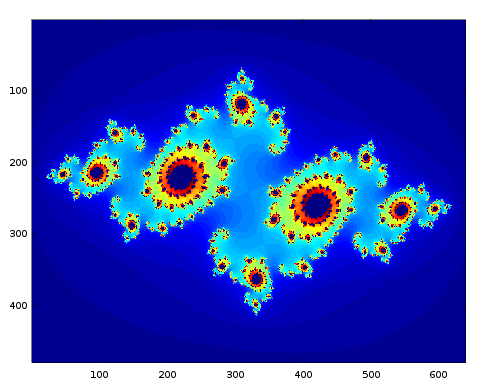
\includegraphics[width = 0.8\textwidth]{img/JuliaOctave.png}
\caption{Conjunto de Julia obtenido mediante Octave}
\label{fig:JuliaOctave}
\end{figure}
\end{minipage}
\begin{minipage}{0.48\textwidth}
\begin{figure}[hbtp]
\centering
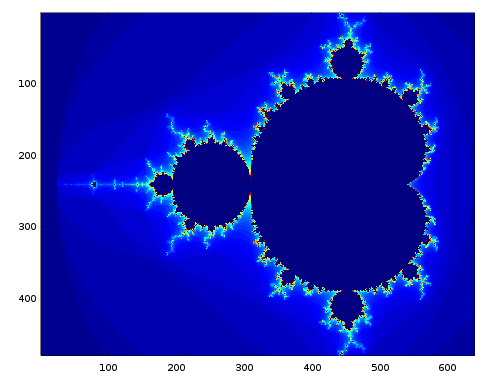
\includegraphics[width = 0.8\textwidth]{img/mandelbrotOctave.png}
\caption{Conjunto de Mandelbrot obtenido mediante Octave}
\label{fig:MandelbrotOctave}
\end{figure}
\end{minipage}
\end{frame}


\subsection{Caos y criptografía}

\begin{frame}
\begin{itemize}
\item La criptografía se ocupa de los problemas de la seguridad de la información y sus pertinentes almacenamientos y transferencias.
\item Un problema caótico muy sensible a los datos iniciales es interesante para la criptografía.
\item Los sistemas caóticos son probabilísticamente difíciles.
\end{itemize}

\begin{block}{Criptografía fractal}
La criptografía fractal o caótica aplica fractales y sistemas caóticos para obtener métodos criptográficos.
\end{block}
\end{frame}

\subsubsection{Usando una función caótica pare encriptar}

\begin{frame}

\begin{block}{Conjunto difuso}
Un subconjunto difuso, es un conjunto que puede contener elementos de forma parcial, es decir que la propiedad  $x\in A$ puede ser cierta, falsa o solamente posible.

Cada elemento tiene una probabilidad asociada.
\end{block}

\begin{example}[Cifrado por bloques simple]
Este es un algoritmo de cifrado por bloques con una clave secreta. La clave es utilizada para generar un pad que luego es combinado con el texto en claro por bloques de 8 bits.

\begin{figure}[hbpt]
\centering
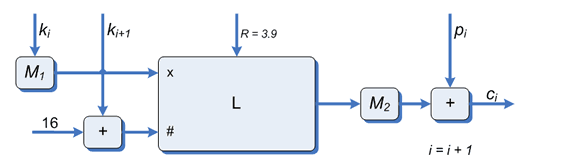
\includegraphics[width = 0.8\textwidth]{img/cifradoCaotico.png}
\end{figure}
\end{example}
\end{frame}

\begin{frame}
\begin{figure}[hbpt]
\centering
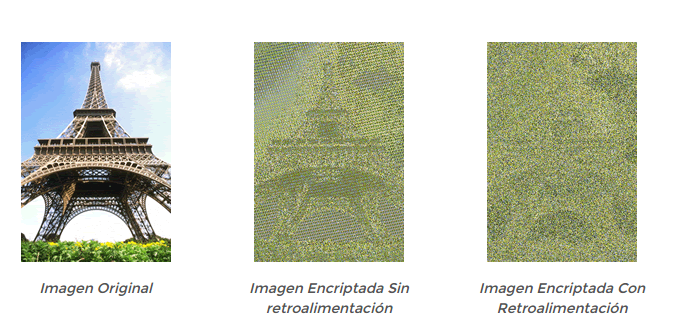
\includegraphics[width = \textwidth]{img/imagenCifradaRetro.png}
\caption{Comparación de imagen original con su versión cifrada y su versión con el cifrado mejorado}
\label{fig:ImagenCifradaRetro}
\end{figure}
\end{frame}

\subsection{Compresión fractal}
\begin{frame}
\begin{block}{Compresión fractal}
La idea básica detrás de la compresión fractal de imágenes, es expresar la imagen como un sistema de funciones iteradas (IFS). La imagen puede mostrarse rápidamente, y un zoom proporciona infinitos niveles de detalles fractales (sintéticos).

El problema es cómo generar eficientemente la imagen IFS.
\end{block}

Hay cuatro características de la tecnología IFS que es necesario conocer para entender su situación actual:
\begin{itemize}
\item Es un método de compresión que pierde un poco de información (como JPG).
\item La resolución al agrandar es poderosa, pero no una forma de comprimir 100:1.
\item La compresión es lenta, la descompresión es rápida.
\item La tecnología está patentada.
\end{itemize}

\end{frame}

\begin{frame}
La idea es tomar una imagen y llevarla a un sistema de funciones iterado, que podría generar el original. No obstante este problema aun no se ha resuelto.

\textbf{Aproximación a la solución}
\begin{itemize}[<+(1)->]
\item En 1988 Barnsley anuncia que resuelve el problema
\item El programa tardaba unas 100 horas por imagen
\item Requería una persona guiando el proceso
\item Comprensión total 10.000:1
\item Posteriormente desarrolla \textbf{Sistema de Funciones Iteradas Particionado (PIFS)}
\item Comprime automáticamente una imagen en un \emph{Sistema de Funciones Iterado Particionado}
\item Una imagen de colores en 24-bit se comprime a 8:1 ó 50:1
\item Actualmente la técnica de compresión fractal no supera el estándar de compresión de imágenes JPEG ni el JPEG2000.
\end{itemize}
\end{frame}

\subsection{Antenas fractales}

\begin{frame}
En la pasada década, los científicos han comenzado a aplicar los fractales a un tema algo \emph{oscuro}: el diseño de las antenas.

\begin{itemize}
\item Aunque las antenas parecen simples tienen una base teórica detrás muy compleja.
\item Los ingenieros de antenas se basan en el método prueba-error
\item Incluso los mejores y más tecnológicos receptores dependen habitualmente de un hilo que no es mejor que el que usó Marconi para la radio hace cien años
\end{itemize}

\textbf{Utilidad de los fractales}
\begin{itemize}
\item Muchas antenas parecen estar compuestas de una unidad independiente, incluyendo la mayoría de antenas de radar, pero en realidad están compuestas de formaciones de cientos de pequeñas antenas [estructura fractal]
\item Colocación de las antenitas en forma fractal combina la robustez de una colocación aleatoria y la eficiencia de una ordenación coherente. [Dwight Jaggard]
\end{itemize}

\begin{center}
``Los fractales son el puente que llena los hueco", comenta Jaggard, ``tienen un desorden a corto alcance y un orden a largo alcance".
\end{center}
\end{frame}

\subsection{Teoría del Caos y Aeronaútica}
\begin{frame}
\begin{block}{Estabilidad vs. Inestabilidad }
\begin{itemize}
\item Búsqueda de estabilidad, evitando entrar en pérdida.
\item Inestabilidad: búsqueda de atractores.
\end{itemize}
\end{block}
\begin{figure}[hbtp]
\centering
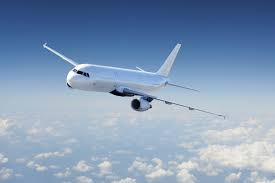
\includegraphics[width = 0.4\textwidth]{img/aero.jpeg}
\caption{Los aviones vuelan en el límite entre la estabilidad y el caos.}
\label{fig:aviones}
\end{figure}
\end{frame}


%------------------------------------------------

\begin{frame}
\frametitle{Fin de la presentación}
\Huge{\centerline{¿Preguntas?}}
\end{frame}

%----------------------------------------------------------------------------------------

\end{document}